\documentclass{erauthesis}
\department{Mechanical Engineering}
\chair{Eric Coyle, Ph.D}
\dean{James Gregory, Ph.D.}
\dgc{Lon Moeller, J.D.}
\depchair{Patrick Currier, Ph.D.}
\advisortitle{Committee chair}
\usepackage{graphicx}
\usepackage{amsmath}
\usepackage{amssymb}
\usepackage{gensymb}
\usepackage{array}
\usepackage{enumitem}
\usepackage{xcolor}
\usepackage{algorithm}
\usepackage{algpseudocode}


\usepackage{subcaption} % for multiple image figures
% \usepackage[style=authoryear]{biblatex} % or numeric, apa, etc.
% \addbibresource{Dissertation.bib}         % your Zotero export

% acronyms
\usepackage{acronym} 

\title{A STUDY IN OBJECT DETECTION AND CLASSIFICATION
PERFORMANCE BY SENSING MODALITY FOR AUTONOMOUS
SURFACE VESSELS} % the title should be included here
\author{Daniel P. Lane} 
\graduation{December}{2025}
\advisor {Eric Coyle} %Committe chair


\coadvisor{Subhradeep Roy} % If you do not have a co-advisor, delete this whole command

\committememzero{Xxxx X. Xxxxxxxxx, Ph.D.} % If you have a co-advisor, do not edit this member name
%% Enter the name of the committee members
\committememone{Patrick Currier}
\committememtwo{Monica Garcia}
\committememthree{Jianhua Liu}
\committememfour{TBD}



%\signaturepush{-2.0}									

\begin{document}

\frontmatter

\maketitle

% \makesignature
\makeatletter 
\advance\fau@frontstage by 1  % Skip signature page but maintain counter
% \makeanother
\begin{acronym}[GB-CACHE] % Give the longest label here so that the list is nicely aligned
\acro{ASV}{Autonomous Surface Vessel}
\acro{USV}{Unmanned Surface Vessel}
\acro{ERAU}{Embry-Riddle Aeronautical University}
\acro{GB-CACHE}{Grid-Based Clustering and Concave Hull Extraction}
\acro{GPS}{Global Positioning System}
\acro{WAM-V}{wave-adaptive modular vessel}
\acro{HDR}{High Dynamic Range}
\acro{IMU}{Inertial Measurement Unit}
\acro{INS}{Inertial Navigation System}
\acro{IoU}{Intersection over Union}
\acro{LiDAR}{Light Detection and Ranging}
\acro{mAP}{mean Average Precision}
\acro{MPC}{model predictive control}
\acro{RGB}{Red, Green, Blue}
\acro{ROI}{Region of Interest}
\acro{ROS}{Robot Operating System}
\acro{USV}{Unmanned Surface Vessel}
\acro{YOLO}{You Only Look Once}
\acro{YOLOv8}{You Only Look Once ver. 8.0}
\acro{LWIR}{Long-Wave Infrared}
\acro{FPS}{Frames per Second}
\acro{EFL}{effective focal length}
\acro{FOV}{Field of View}
\acro{LAN}{Local Area Network}
\acro{SEI}{Supplemental Enhancement Information}
\acro{NAL}{Network Abstraction Layer}
\acro{NTP}{Network Time Protocol}
\acro{PTP}{Precision Time Protocol}
\acro{RTP}{Real-time Transport Protocol}
\acro{RTSP}{Real-time Streaming Protocol}
\acro{UDP}{User Datagram Protocol}

\end{acronym}

\begin{acknowledgements}

	% \raggedright XXxxxx xxxxx xxxxx xxxxx xxxxx xxxxx xxxxx.  Xxxxx xxxxx xxxxx xxxxx xxxxx xxxxx xxxxx xxxxx xxxxx xxxxx xxxxx xxxxx xxxxx xxxxx xxxxx xxxxx xxxxx xxxxx.\\Xxxxx xxxxx xxxxx xxxxx xxxxx xxxxx xxxxx xxxxx xxxxx xxxxx xxxxx xxxxx xxxxx xxxxx xxxxx xxxxx xxxxx xxxxx xxxxx xxxxx.  Xxxxx xxxxx xxxxx xxxxx xxxxx xxxxx xxxxx xxxxx xxxxx xxxxx xxxxx xxxxx xxxxx xxxxx xxxxx.\\
    \raggedright In addition to any personal statements of acknowledgement, be sure to include any acknowledgement statements required by research sponsors.\\{[Single page limit]} 

    \raggedright This research was sponsored in part by the Department of the Navy, Office of Naval Research through ONR N00014-17-1-2492, and the Naval Engineering Education Consortium (NEEC) through grants N00174-19-1-0018 and N00174-22-1-0012, sponsored by NSWC Carderock and NUWC Keyport, respectively. Any opinions, findings, conclusions, or recommendations expressed in this material are those of the authors and do not necessarily reflect the views of the Department of the Navy or Office of Naval Research.
\end{acknowledgements}

\begin{abstract}
	\raggedright Researcher: Daniel P. Lane
 \\Title: A study in object detection and classification performance by sensing modality for autonomous surface vessels \\Institution:	Embry-Riddle Aeronautical University\\Degree:	Doctor of Philosophy in Mechanical Engineering\\Year:	2025 \\
 This research addresses the critical gap in quantitative performance comparison between \ac{LiDAR} and vision-based sensing for real-time maritime object detection on autonomous surface vessels.
 Using \ac{ERAU}'s Minion platform and 2024 Maritime RobotX Challenge data, this study evaluates \ac{GB-CACHE} \ac{LiDAR} processing against \ac{YOLO} vision detection across six maritime object categories. The methodology encompasses real-time performance analysis, multi-sensor calibration, and sensor fusion for bounding box confidence integration.
 Performance metrics include precision, recall, \ac{mAP}, training requirements, and computational efficiency. 
 % Results demonstrate [key performance finding] and establish [fusion outcome]. 
 The research provides quantitative baselines for maritime sensing modality selection and validated calibration procedures enabling improved autonomous navigation in complex maritime environments.
 
 % Lorem ipsum dolor sit amet... This is a summative abstract, not just a list of topics.  Include relevant information including conclusions and recommendations.  Limit to 150 words; spell out abbreviations; citations not needed.

\end{abstract}
\pagetableofcontents
\clearpage
\listoftables					% Or \nolistoftables if there are no 
\clearpage
\listoffigures					% Or \nolistoffigures if there are no 



\mainmatter
\newpage
\chapter{Introduction} 

\section{Introduction} \label{introduction}

\subsection{Significance of Study} \label{significance_of_study}

The development of \acp{ASV} represents a significant technological advancement requiring sophisticated perception systems capable of detecting and classifying maritime objects with high accuracy and reliability in real-time operational environments. As \ac{ASV} technology advances toward practical deployment in commercial and research applications, understanding the comparative performance characteristics of different sensing modalities and their integration through sensor fusion methodologies becomes critical for effective system design and operational safety assurance.

The advancement of autonomous surface vessel technology has gained significant momentum through comprehensive research programs and competitive evaluation platforms such as the Maritime RobotX Challenge, where multidisciplinary teams develop and test \ac{ASV} platforms under realistic maritime operational conditions. These research platforms serve as essential testbeds for evaluating perception technologies under actual environmental constraints, providing valuable empirical insights into sensor performance characteristics, real-time processing capabilities, and complex system integration challenges that cannot be adequately assessed through simulation alone.

Research platforms provide critical opportunities for real-world validation of perception algorithms under actual maritime conditions with operational time constraints. These platforms enable comprehensive comparative analysis opportunities for evaluating different sensor modalities and advanced sensor fusion approaches under controlled yet realistic testing scenarios. Furthermore, research platforms facilitate essential technology transfer pathways from experimental research systems to operational \ac{ASV} deployments requiring robust real-time performance guarantees. Finally, these platforms enable systematic performance benchmarking that supports rigorous evaluation of detection accuracy, classification reliability, and sensor fusion effectiveness across diverse maritime operational scenarios.

Current \ac{ASV} development faces a significant knowledge gap regarding the quantitative performance characteristics of different sensing modalities and their integration methodologies in complex maritime environments. While individual sensor technologies, particularly \ac{LiDAR} systems and vision-based cameras, have been extensively studied and validated in terrestrial applications, their comparative performance characteristics and sensor fusion integration capabilities in maritime contexts lack systematic quantitative analysis with emphasis on real-time processing constraints and computational efficiency requirements.

Comprehensive performance analysis requires systematic detection accuracy comparison between \ac{LiDAR}-based systems utilizing \ac{GB-CACHE} processing and vision-based systems implementing \ac{YOLO} object detection algorithms. Additionally, rigorous classification performance evaluation across diverse maritime object types using advanced machine learning algorithms must be conducted to establish performance baselines. Assessment of training requirements for machine learning-based classification systems, particularly focusing on data efficiency and convergence characteristics, represents another critical analytical requirement. Real-time processing capabilities and computational efficiency evaluation under operational constraints must be systematically analyzed to ensure practical deployment feasibility. Moreover, sensor fusion effectiveness evaluation, specifically examining bounding box confidence integration methodologies, requires a comprehensive analysis to determine optimal multi-modal processing approaches. Finally, environmental robustness evaluation across varying maritime conditions, including different weather states, lighting conditions, and sea states, must be conducted to ensure reliable operational performance.

\ac{ASV} perception systems must reliably detect and classify a diverse range of maritime objects that are critical for safe autonomous navigation, requiring robust algorithms capable of real-time processing under challenging environmental conditions. The maritime environment presents unique detection challenges due to varying lighting conditions, wave-induced platform motion, and the diverse physical characteristics of navigation-critical objects that must be accurately identified and classified. Navigation buoys, including Polyform A-2 and A-3 buoys available in various colors for channel marking and navigation guidance, represent primary detection targets requiring high accuracy classification. Regulatory markers, specifically Sur-Mark tall buoys designed for navigation reference and hazard identification, present distinct detection challenges due to their geometric characteristics and operational deployment contexts. Light towers serving as active navigation aids provide both visual and electronic guidance signals, requiring detection algorithms capable of handling variable illumination and signaling states. Various vessels, including recreational boats and commercial watercraft, represent dynamic detection targets with diverse sizes, shapes, and motion characteristics that complicate reliable classification. Maritime infrastructure elements, including docks, piers, and other fixed navigational hazards, require robust detection capabilities to ensure safe autonomous navigation in complex harbor and coastal environments.

% \subsection{Problem Statement}
\subsection{Problem Statement: Performance Comparison Gap} \label{problem_statement1}

Despite the growing operational importance of autonomous surface vessels and the significant maturation of individual sensor technologies over the past decade, there exists a critical and well-documented gap in quantitative performance comparison between different sensing modalities specifically applied to maritime object detection and classification tasks. Current \ac{ASV} development efforts lack systematic analytical frameworks for evaluating how \ac{LiDAR}-based systems utilizing advanced point cloud processing algorithms perform relative to vision-based systems implementing state-of-the-art deep learning approaches when deployed in realistic maritime operational environments.

Existing research efforts in maritime object detection and classification have primarily focused on individual sensor implementations and algorithm development without conducting a comprehensive comparative analysis that would inform optimal sensor selection and integration strategies for operational \ac{ASV} systems. Contemporary research demonstrates a predominant focus on \ac{LiDAR}-only implementations that emphasize point cloud processing methodologies and clustering algorithms specifically adapted for maritime environments, yet these studies typically lack comparative evaluation against alternative sensing modalities. Similarly, vision-only system research emphasizes deep learning approaches for maritime object recognition, particularly convolutional neural network architectures, but generally operates in isolation without systematic comparison to \ac{LiDAR}-based approaches. The limited cross-modal comparison studies that do exist provide insufficient quantitative performance metrics and lack standardized evaluation frameworks necessary for meaningful comparative analysis. Furthermore, there exists a notable absence of standardized evaluation frameworks specifically designed for maritime perception systems, hindering systematic comparison and technology advancement across research groups and commercial developers.

The absence of comprehensive quantitative performance analysis leaves fundamental technical and operational questions unanswered for \ac{ASV} system designers and engineers responsible for developing reliable autonomous navigation systems. Critical questions regarding detection and classification performance remain inadequately addressed in current research literature. Specifically, the comparative detection accuracy performance of \ac{LiDAR}-based systems utilizing \ac{GB-CACHE} processing versus vision-based systems implementing \ac{YOLO} algorithms for specific maritime object types requires systematic investigation. The precision and recall characteristics of each sensing modality across different object classes under varying environmental conditions need quantitative evaluation to inform sensor selection decisions. Training requirements, including data volume, computational resources, and convergence time, differ significantly between \ac{LiDAR} feature-based approaches and vision-based deep learning methodologies, yet these differences lack systematic quantification. Computational overhead associated with each sensing modality for real-time operation, including processing latency and resource utilization, requires comprehensive analysis to ensure practical deployment feasibility. Additionally, the effectiveness of sensor fusion methodologies, particularly bounding box confidence integration approaches, needs rigorous evaluation to determine optimal multi-modal processing strategies for enhanced detection performance.

% \subsection{Problem Statement}
\subsection{Problem Statement: Sensor Fusion Challenges} \label{problem_statement2}

Autonomous surface vessels require precise integration of multiple sensing modalities to achieve reliable object detection and classification performance that meets operational safety standards for autonomous navigation. A fundamental and persistent challenge in \ac{ASV} perception system development lies in establishing and maintaining accurate spatial and temporal calibration between \ac{LiDAR} and camera systems under dynamic maritime operational conditions that present unique environmental challenges not encountered in terrestrial applications.

Multi-sensor \ac{ASV} platforms face unique spatial calibration requirements that differ significantly from terrestrial applications due to the dynamic nature of maritime environments and the continuous mechanical stresses imposed by marine operational conditions.
Environmental factors affecting calibration present ongoing challenges for maintaining sensor alignment accuracy. Platform motion induced by wave action creates continuous roll, pitch, and yaw movements that affect sensor alignment and require robust calibration maintenance strategies. Vibration and mechanical stress inherent in marine environments cause gradual calibration drift that can degrade sensor fusion performance over extended operational periods. Temperature variations in maritime environments affect sensor mounting structures and optical characteristics, potentially introducing systematic calibration errors that must be compensated through adaptive calibration procedures. Saltwater corrosion presents long-term challenges by potentially altering sensor mounting hardware characteristics over extended deployment periods, requiring regular calibration, validation, and maintenance protocols.

Precision requirements for effective sensor fusion establish demanding performance specifications for calibration maintenance systems that must operate reliably under dynamic maritime conditions. Sub-pixel accuracy calibration is essential for accurate \ac{LiDAR} point cloud projection onto camera images, enabling effective correlation between sensor modalities for object detection applications and ensuring that spatial relationships between sensors remain consistent across operational scenarios. Millimeter-level precision in spatial calibration is required for effective object detection correlation between \ac{LiDAR} and vision systems, particularly for small maritime objects such as navigation buoys, where detection accuracy directly impacts navigation safety. Consistent calibration maintenance across varying operational conditions, including different sea states and weather conditions, requires robust calibration validation procedures that can adapt to changing environmental parameters. Real-time calibration validation capabilities are necessary for detecting calibration degradation during operation and implementing corrective measures to maintain sensor fusion performance without interrupting autonomous navigation operations.

\subsection{Limitations and Assumptions} \label{limitations}

This research investigation is conducted using \ac{ERAU}'s Minion \ac{ASV} research platform and utilizes sensor data collected during the 2024 Maritime RobotX Challenge competition, which establishes specific operational and methodological constraints that define the scope and applicability of research findings.

Platform-specific limitations inherent in this research approach must be acknowledged and considered when interpreting results and their broader applicability. Research findings are specifically applicable to \ac{ERAU}'s Minion research platform design, including its particular sensor mounting configuration, platform dynamics characteristics, and operational capabilities, which may not directly translate to other \ac{ASV} platform designs. The competition environment context, where primary data collection occurred during RobotX challenge events, may not represent the full spectrum of maritime operational conditions encountered in commercial or military \ac{ASV} deployments. Geographic constraints imposed by conducting testing in competition and training areas introduce environmental characteristics that may not be representative of other maritime operational regions. Operational scenarios focused on RobotX challenge tasks may not encompass the complete range of potential \ac{ASV} mission requirements and environmental conditions encountered in practical autonomous vessel operations.

This research focuses on specific maritime object categories that are relevant to RobotX competition scenarios and representative of typical \ac{ASV} navigation challenges, while acknowledging that maritime environments contain additional object types not addressed in this investigation. The research addresses six primary object classes that represent critical navigation elements in maritime environments. Tall buoys, specifically Sur-Mark regulatory buoys with standardized dimensions of 39-inch height, 10-inch column diameter, and 18-inch ring diameter, represent regulatory navigation markers requiring reliable detection and classification. Polyform A-2 buoys, measuring 14.5 inches by 19.5 inches and available in red, green, blue, and black color variants, serve as channel markers and navigation references requiring color-specific classification capabilities. Polyform A-3 buoys, with dimensions of 17 inches by 23 inches and identical color availability, represent larger navigation buoys requiring robust detection across varying distances and environmental conditions. Light towers function as active navigation aids incorporating electronic and visual signaling capabilities, presenting detection challenges due to variable illumination states and complex geometric structures. Jon boats, characterized as flat-bottom chase boats utilized in competition and training scenarios, represent small vessel detection targets with distinct geometric and motion characteristics. Sailboats, including recreational sailing vessels commonly encountered in competition environments, represent larger vessel detection targets with variable configuration due to sail and rigging arrangements.

\textbf{Definitions of Terms}

\begin{itemize}[label={}]
    \item\textbf{Autonomous Surface Vessel (ASV)} An unmanned watercraft capable of independent navigation and task execution without direct human control, utilizing onboard sensors and computational systems for environmental perception and decision-making.
    
    \item\textbf{Clustering} A computational technique that groups data points with similar characteristics or spatial proximity to identify distinct objects or regions within complex datasets.

    \item\textbf{Grid-Based Clustering} A spatial data organization methodology that partitions three-dimensional point cloud data into regular grid structures to facilitate efficient clustering analysis and object identification within defined spatial regions.
    
    \item\textbf{Concave Hull} A geometric boundary that closely follows the shape of a point set by allowing inward curves, providing a more accurate representation of object boundaries compared to convex hull approaches.
    
    \item\textbf{You Only Look Once (YOLO)} A real-time object detection algorithm that processes entire images in a single forward pass through a convolutional neural network, simultaneously predicting bounding boxes and class probabilities for detected objects.
    
    \item\textbf{Sensor Fusion} The computational process of combining data from multiple sensors to produce more accurate, reliable, or comprehensive information than could be achieved using individual sensors independently.
    
    \item\textbf{Bounding Box} A rectangular region that defines the spatial boundaries of a detected object within an image or three-dimensional space, typically specified by corner coordinates or center point with width and height dimensions.
    
    \item\textbf{Confidence Integration} A methodology for combining detection results from multiple sensors by evaluating and integrating the confidence scores associated with object predictions to improve overall detection reliability.
    
    \item\textbf{Maritime RobotX Challenge} An international autonomous surface vessel competition that provides standardized testing scenarios and performance evaluation frameworks for ASV perception, navigation, and manipulation capabilities.
    
    \item\textbf{Real-time Processing} Computational processing that guarantees response within specified time constraints, typically requiring completion of detection and classification tasks within predetermined latency limits suitable for autonomous navigation safety requirements.
    
    \item\textbf{Light Detection and Ranging (LiDAR)} A remote sensing technology that uses laser pulses to measure distances and create detailed three-dimensional point cloud representations of environmental features and objects.
    
    \item\textbf{Point Cloud} A collection of data points in three-dimensional space representing the external surface of objects, typically generated by LiDAR sensors through distance measurements to environmental features.
\end{itemize}

\textbf{List of Acronyms}

\begin{itemize}[label={}]
    \item\textbf{ASV} Autonomous Surface Vessel
    \item\textbf{ERAU} Embry-Riddle Aeronautical University  
    \item\textbf{GB-CACHE} Grid-Based Clustering and Concave Hull Extraction
    \item\textbf{LiDAR} Light Detection and Ranging
    \item\textbf{RGB} Red, Green, Blue
    \item\textbf{ROS} Robot Operating System
    \item\textbf{YOLO} You Only Look Once
    \item\textbf{IoU} Intersection over Union
    \item\textbf{mAP} mean Average Precision
    \item\textbf{ROI} Region of Interest
    \item\textbf{GPS} Global Positioning System
    \item\textbf{IMU} Inertial Measurement Unit
\end{itemize}

%%%%%%%%%%%%%%%%%%%%%%%%%%%%%%%%%%%%%%%%%%%%%%%%%%%%%%%%%%%%%%%%%%%%
%%%%%%%%%%%%%%%%%%%%%%%%%%%%%%%%%%%%%%%%%%%%%%%%%%%%%%%%%%%%%%%%%%%%
%%%%%%%%%%%%%%%%%%%%%%%%%%%%%%%%%%%%%%%%%%%%%%%%%%%%%%%%%%%%%%%%%%%%
\chapter{Review of the Relevant Literature} \label{litReview}

% Note: All in-text citations should appear as \cite{einstein}

\acp{USV} have emerged as essential platforms capable of performing dangerous, dirty, and cumbersome tasks that exceed human capability. These vessels are pivotal in various maritime operations, including environmental monitoring, search and rescue missions, and resource exploration \cite{liebergall, eckstein2024}.% [1], [2]. 
Their ability to operate independently with minimal human intervention has significantly enhanced operational efficiency and safety at sea \cite{bai2022}.%[3].

Autonomous vehicles use a variety of sensors to perceive their surroundings, but primarily rely on some combination of visual information through a camera and spatial data provided by \ac{LiDAR} \cite{yeong2021}.%[4].
Each sensing modality offers distinct advantages: visual data provides rich color and texture information, while \ac{LiDAR} delivers precise spatial measurements of the surrounding environment.
Real-time object detection methods have been developed for both sensing modalities, leveraging deep learning architectures.
Object detection with visual data often employs transfer learning on pre-trained convolutional neural networks such as ResNet \cite{he2016} and \ac{YOLO} \cite{ultralytics}.%[6].
Similarly, \ac{LiDAR}-based object detection can be performed using point-based algorithms like PointNet \cite{garcia-garcia2016}, voxel-based methods such as VoxelNet \cite{zhou2018a}, or hybrid approaches like PV-RCNN \cite{shi2021}.%[9].
Despite these advancements, each modality has inherent limitations—vision-based systems struggle with poor lighting conditions and occlusions, while \ac{LiDAR} data can be sparse and affected by water reflections.

To address these limitations, sensor fusion techniques have been explored as a means of combining the strengths of both modalities. 
Research into sensor fusion methods dates back to military applications in the 1980s and has gained significant traction in the last 15 years, particularly due to interest from the automotive industry in autonomous driving technologies. However, no unified approach has been established for optimal sensor fusion, with ongoing debates regarding the best fusion strategies (e.g., early, mid, or late fusion) and their trade-offs concerning computational efficiency and accuracy.

While research in the automotive sector has contributed significantly to sensor fusion methodologies \cite{yeong2021,clunie2021,roriz2022,cui2022,das2022,liu2023a}, direct application to maritime environments remains challenging due to fundamental environmental differences. 
Automotive environments are highly structured, with well-defined lanes, uniform object classes, and relatively predictable lighting conditions. 
In contrast, the maritime environment introduces additional complexities, including dynamic vehicle motion induced by wind and waves, variable scene density (ranging from sparse open waters to congested littoral zones), and specular reflections on the water surface that can interfere with both vision-based \cite{liu2023a} and \ac{LiDAR}-based object detection \cite{ahmed2024}.%[15]. 
These factors necessitate domain-specific adaptations of sensor fusion architectures to ensure robust real-time object detection for \acp{USV}. 
However, the lack of available maritime-specific datasets \cite{jun-hwa2022,su2023,thompson2023} creates an additional challenge.

Given these challenges, further research is needed to enhance sensor fusion methodologies for maritime applications. 
Key areas of investigation include efficient feature selection tailored to maritime object classes, the development of lightweight fusion architectures suited for real-time processing, and an evaluation of computational requirements for deployment on \ac{USV} hardware. 
Addressing these research gaps will contribute to the advancement of autonomous maritime perception, enhancing the operational capabilities of \acp{USV} in complex and dynamic environments.

\chapter{Sensing Platform and Data Acquisition} \label{sensing_platform}
\section{System Overview}
% % \textcolor{red}{This intro section should provide an overview of the Minion USV platform and related sub-systems: Atlas, Camera Enclosure}
% The Minion \Ac{ASV} is a maritime research vessel developed by \ac{ERAU} to provide graduate-level research and undergraduate hands-on learning opportunities, as well as to compete in the Maritime RobotX Challenge, and served as the primary research platform for the research in this paper.
% The platform is based upon a \ac{WAM-V} equipped with a comprehensive suite of \ac{LiDAR}, infrared and visual spectrum cameras, \ac{GPS}, and \acp{IMU} designed to support navigation and perception research, allowing Minion to operate autonomously within littoral zones and open water.

% A dual-antenna \ac{GPS} is paired with three 360-degree  \ac{LiDAR} units placed around Minion's top deck to provide the omnidirectional awareness required for autonomous navigation.
% An additional three forward scanning \ac{LiDAR} sensors optimize point cloud density in the forward direction of travel.
% The same point-dense \ac{FOV} \ac{LiDAR} cloud off of Minion's bow is also spanned by a suite of six cameras mounted within a water-tight camera enclosure.
% Camera data is processed within the camera enclosure on an NVIDIA Jetson Xavier, equipped with hardware-accelerated video drivers capable of compressing and streaming all six video feeds over the robot's gigabit \ac{LAN}.

% Atlas is Minion's brain and network back-bone designed in 2018. 
% It houses a single gigabit 16-port network switch and a twin PC architecture for redundancy, each possessing computing power equivalent to a high-end smart-phone in 2025.

% Each PC and all sensor data is synchronized the robot's \ac{LAN} through \ac{NTP} and \ac{PTP} signals originating from the \ac{GPS} clock.

% Finally all of this information is processed on one of the two twin Minion PCs by fully custom software written by \ac{ERAU} students and synthesized with \ac{ROS}, culminating in a robust platform for maritime perception research. 
% The original sensor selection and configuration detailed in this chapter was developed by \acp{ERAU} Team Minion for the 2022 and 2024 Maritime RobotX Competition \cite{holland2024} \cite{thompson2023}.% \cite{lachguar}. 

% This chapter details the technical specifications of full complement of hardware onboard Minion, with greater detail provided to the LiDAR and high definition cameras within the camera enclosure.
% Additionally, a discussion of visual spectrum sensors and  selection can be found in \ref{visual_cameras}
% The primary enhancement to the sensor suite introduced by this work is a timestamp embedding mechanism robust to network delay, detailed in Section~\ref{video pipeline}, which is essential for rigorous multi-modal sensor fusion analysis.

% The Minion \Ac{ASV} is a maritime research vessel developed by \ac{ERAU} as a platform for graduate-level research, undergraduate experiential learning, competition in the Maritime RobotX Challenge, as well as the primary research platform for the work presented in this dissertation.
The Minion \Ac{ASV} serves as a multidisciplinary platform for undergraduate instruction and graduate research at \ac{ERAU}.
Built on a \ac{WAM-V} hull, the platform integrates a comprehensive sensor suite including \ac{LiDAR}, visual and infrared cameras, \ac{GPS}, and \acp{IMU} to enable autonomous operation in both littoral zones and open-water environments.
Figure \ref{fig:minion} shows a render of the vessel as it was equipped to compete in the 2024 Maritime RobotX Challenge, as well as the data collection necessary to conduct the research presented in this dissertation.

The platform's sensing architecture provides omnidirectional environmental awareness with a dual-antenna \ac{GPS} along with three strategically placed 360-degree \ac{LiDAR} units.
Three additional forward-scanning \ac{LiDAR} sensors are paired with a suite of six cameras to provide enhanced point cloud density and high-resolution visual data in the vessel's primary direction of travel. 
% Within this forward-facing \ac{FOV}, a suite of six cameras provides high-resolution visual data housed within a watertight enclosure.
Video processing from these cameras occurs locally within the watertight camera enclosure on an NVIDIA Jetson Xavier module.
This PC performs the hardware-accelerated compression necessary to stream all six feeds over the vessel's \ac{LAN}.

% Minion's main computer, designated Atlas, was designed in 2018 to serve as the vessel's central processing hub and network backbone. 
The Atlas computing system, developed in 2018, serves as the \acp{USV} central processing unit and network backbone.
Comprised of a 16-port network switch and a redundant twin-PC architecture, Atlas is manages synchronization across all network endpoints and sensors while performing high-level data processing.
% and facilitating sensor communication.and is capable of processing all of the captured data in near real-time on hardware comparable to a contemporary smartphone.
% Temporal synchronization across all sensors and network endpoints is maintained via \ac{NTP} and \ac{PTP} protocols referenced to the \ac{GPS} clock signal. 
The integrated software stack was developed by \ac{ERAU} Faculty and students and is built upon the \ac{ROS} framework and processes the multi-sensor data stream in near real-time to enable autonomous maritime operations.

% The sensor configuration described in this chapter was originally developed by Team Minion for the 2022 and 2024 Maritime RobotX competitions \cite{holland2024, thompson2023}. This chapter presents the technical specifications of Minion's complete hardware complement, with particular emphasis on the \ac{LiDAR} sensors and high-definition cameras housed within the forward camera enclosure. Section~\ref{visual_cameras} provides additional discussion regarding visual spectrum sensor selection and characterization. The primary contribution of this work to the existing sensor suite is a network-delay-robust timestamp embedding mechanism, detailed in Section~\ref{video pipeline}, which enables precise temporal alignment essential for rigorous multi-modal sensor fusion analysis.

\begin{figure}[t]
\centering
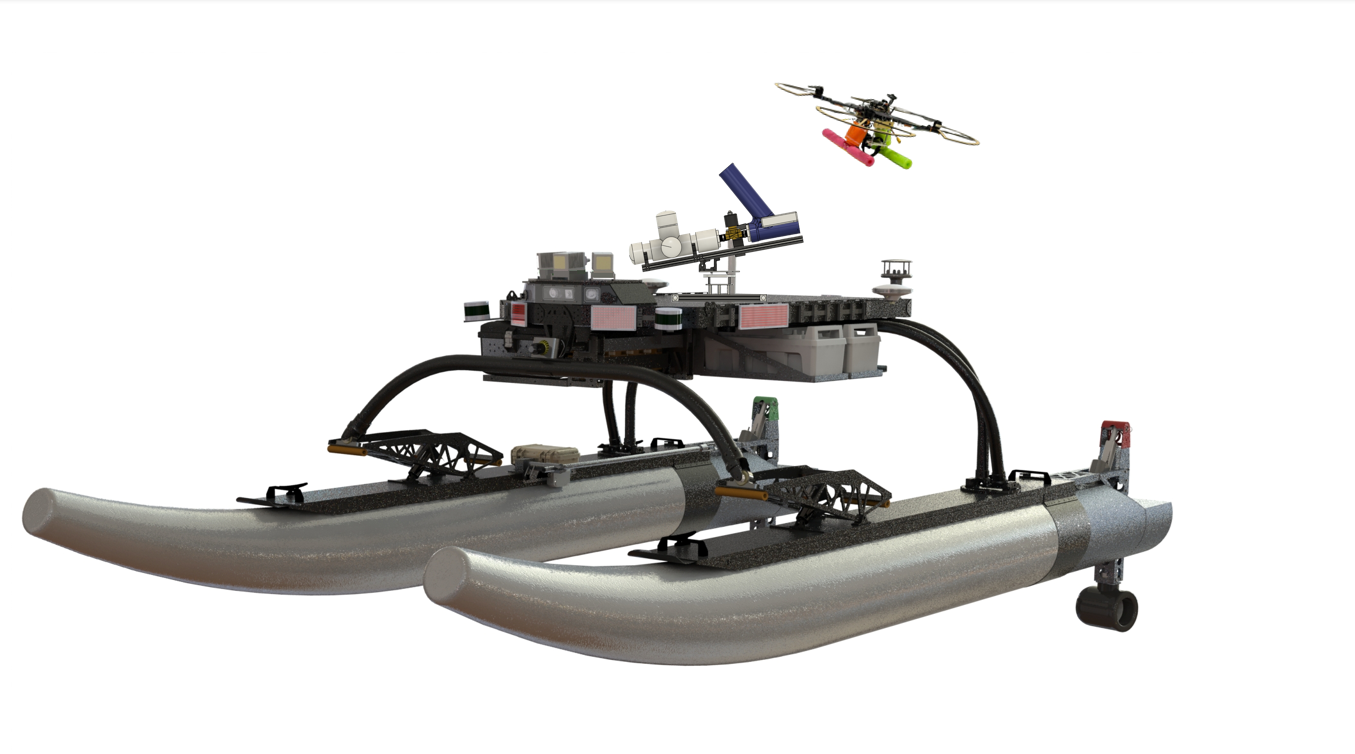
\includegraphics[width=0.8\textwidth]{Images/Minion.png}
\caption{ERAU's \ac{WAM-V} Research Vessel Minion as configured for the 2024 Maritime RobotX Challenge.}
\label{fig:minion}
\end{figure}

The sensor configuration described in section~\ref{perception_geometry} was originally developed by Team Minion for the 2022 and 2024 Maritime RobotX competitions \cite{holland2024, thompson2023}. Section~\ref{sensors} presents the technical specifications of Minion's sensor hardware, with particular emphasis on the \ac{LiDAR} and high-definition camera sensors selected for this study.
An overview of the CPU and network infrastructure of the system is provided in section~\ref{sec:Atlas_LAN} as background for the computational requirements of the real-time object detection methods presented in Chapter~\ref{object-detection}, as well as the challenges relating to the synchronization of sensors in section~\ref{sec:calibration}.
% housed within the forward camera enclosure. Section~\ref{visual_cameras} provides additional discussion regarding visual spectrum sensor selection and characterization. 
Of particular note, the timestamp embedding mechanism described in Section~\ref{time_sync_cam} overcomes network latency issues in the video pipeline to maintain a more precise temporal alignment.
% , essential for rigorous multi-modal sensor fusion analysis.
Finally, section~\ref{sensor_data} discusses the \ac{ROS} software architecture responsible for recording and processing sensor data.

%%%%%%%%%%%%%%%%%%%%%%%%%%%%%%%%%%%%%%%%%%%%%%%%%%%%%%%%%%%%%%%%%%%%
%%%%%%%%%%%%%%%%%%%%%%%%%%%%%%%%%%%%%%%%%%%%%%%%%%%%%%%%%%%%%%%%%%%%
\section{Perception Geometry} \label{perception_geometry}

Minion is equipped with six \ac{LiDAR} sensors as well as six cameras to perceive her surroundings.
Omnidirectional \ac{LiDAR} coverage is provided by three Velodyne VLP-16 units for situational awareness within the \acp{USV} immediate operating environment.
% \ac{LiDAR} coverage and object detection within the vessel's immediate operating environment.
Three additional forward-scanning Livox Horizon \ac{LiDAR} generate a dense point cloud ahead of the vessel for object detection and classification at greater distances.
The Livox units are directly mounted to a camera enclosure which houses four high-definition visual-spectrum cameras and two \ac{LWIR} cameras.
The combination of forward-scanning LiDAR and cameras provides a significantly higher fidelity of data within a shared 165-degree \ac{FOV}.% in the direction of travel.
% The camera enclosure design emphasizes modularity and research flexibility.
Figure~\ref{fig:camera_enclosure} presents the mounting location of the Livox Horizon LiDAR units and each of the six cameras within the waterproof enclosure. 

\begin{figure}[htbp]
\centering
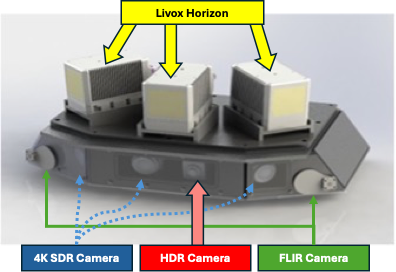
\includegraphics[width=0.6\textwidth]{Images/Camera_enclosure2.png}
\caption{Mounting locations of three Livox Horizon LiDAR units (yellow arrow, top) two LWIR cameras (green, thin, solid arrows), three FLIR 4k cameras (blue, dotted arrows), and a single \ac{HDR} camera  (red arrow, bottom) within the camera enclosure.}
\label{fig:camera_enclosure}
\end{figure}

% While the Velodyne \ac{LiDAR} sensors provide comprehensive 360-degree environmental awareness for navigation and collision avoidance, the three forward-facing Livox Horizon \ac{LiDAR} units mounted to the camera enclosure were selected for their superior point cloud density and ability to facilitate a higher resolution for object detection.
% The three Livox units concentrate sampling density in the forward \ac{FOV}, matching the horizontal coverage of the six cameras.
% Both modalities overlap the \ac{FOV} of their respective individual sensors.
% This sensor arrangement ensures higher density and more uniform point-cloud across the 165-degree forward perception envelope in the case of \ac{LiDAR}, but also makes the system more robust to failure.
% Losing a single sensor will not create a blind spot for either sensing modality in the forward path of motion of the \ac{USV}. 
% Figures~\ref{fig:fov_cam} and ~\ref{fig:fov_lidar} show how the horizontal \ac{FOV} for each of these sensors overlaps in the direction of travel.

% Each of these sensors is installed so that the center of their \ac{FOV} is parallel to one of three separate lines of vision.
% The first of these lines is a vector that points down the centerline of the vessel in the forward direction, and sensors in this orientation receive the moniker of \texttt{sensor\_center}.
% The other two lines of vision are rotated 40 degrees counterclockwise and clockwise from the centerline, and sensors in these orientations receive the moniker \texttt{sensor\_port} and \texttt{sensor\_starboard}, respectively.
Each sensor’s optical axis is aligned with one of three predefined sight lines: the vessel's centerline and two axes rotated $\pm 40$ degrees from the center.
% In the case of LiDAR, this sensor arrangement provides a denser point cloud and, in general, means that the loss of signal from any single sensor does not create a blind spot in the forward direction of travel.
For the LiDAR system, this configuration increases point-cloud density in the forward direction and ensures that loss of any single sensor does not produce a blind spot in the forward direction of travel.
% Figure~\ref{fig:fov_combined} shows the camera's \ac{FOV} in \ref{fig:fov_cam}, and the the LiDAR \ac{FOV} in \ref{fig:fov_lidar}.
Each of the three Livox Horizon LiDAR units has an 81.7-degree \ac{FOV}, resulting in more than a 40-degree overlap in the \ac{FOV} between \texttt{livox\_center} and both \texttt{livox\_port} and \texttt{livox\_starboard}, and approximately 3 degrees of overlap between \texttt{livox\_port} and \texttt{livox\_starboard} (figure~\ref{fig:fov_lidar}).
Three 4K cameras are configured to point in the port, center, and starboard directions. 
While these cameras are equipped with a Theia-TL410P zoom lens, they are currently set at a fixed zoom level that approximates a \textcolor{blue}{(65-degree?)} horizontal \ac{FOV}, which provides a \textcolor{blue}{(32.5-degree)} overlap in their \ac{FOV} (figure~\ref{fig:fov_cam}).
The two \ac{LWIR} cameras each have a 90-degree \acs{FOV}, and are positioned along the port and starboard vision lines, providing a 10-degree overlap.
Finally, there is a single HDR camera with a 65-degree horizontal \ac{FOV} that points forward.
While the \ac{HDR} camera lacks any of the aforementioned sensor redundancy, its \ac{FOV} aligns with the central 4k camera and was added for research that compared the two center-line mounted cameras \cite{liebergall}.

% related to the dynamic range of the two center-line mounted cameras  and was selected as the primary visual range sensor for this body of work for reasons that are discussed in section~\ref{visual_cameras}.


\begin{figure}[htbp]
\centering
\begin{subfigure}[t]{0.48\textwidth}
    \centering
    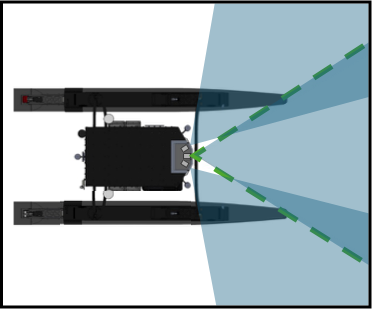
\includegraphics[width=\textwidth]{Images/fov_cam.png}
    \caption{Blue cones represent \ac{FOV} from individual FLIR 4K camera; green dashed lines indicate \ac{FOV} of HDR camera. \textcolor{red}{(This image may need to be re-created. port and sb FOV should not overlap. check fixed FOV)}}
    \label{fig:fov_cam}
\end{subfigure}
\hfill
\begin{subfigure}[t]{0.48\textwidth}
    \centering
    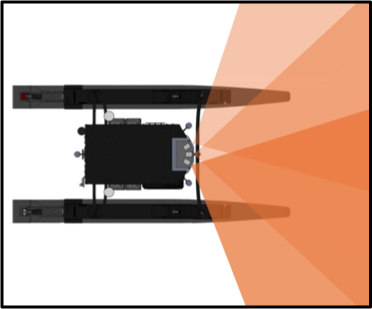
\includegraphics[width=\textwidth]{Images/fov_lidar.png}
    \caption{LiDAR horizontal \ac{FOV} overlap.}
    \label{fig:fov_lidar}
\end{subfigure}
\caption{Comparative visualization of horizontal \ac{FOV} (FOV) overlap for (a) cameras and (b) LiDAR sensors.}
\label{fig:fov_combined}
\end{figure}

% A Torc Robotics PinPoint \ac{GPS}/\ac{IMU} system is equipped with provides both global time synchronization and platform pose estimation.

% The sensor coordinate frames are organized in a hierarchical transformation tree structure, which is shown in \ref{transform_diagm}.
% The inertial reference frame (\texttt{map}) defines the world-fixed coordinate system.
% The platform reference frame (\texttt{base\_link}) represents the vessel body frame defined by the PinPoint \ac{GPS}/\ac{IMU}.
% The center Livox frame (\texttt{livox\_center}) serves as the primary sensor reference frame, with \texttt{livox\_port} and \texttt{livox\_starboard} both reporting data in the \texttt{livox\_center} reference frame.
% Six camera image frames exist within this tree, and are referenced to the \texttt{livox\_center} frame.
% Intrinsic calibration parameters, including camera-specific matrices and distortion coefficients, along with extrinsic transformation parameters relating sensor frames to each other and to the platform frame, are discussed in \textcolor{red}{Appendix \#}.

% The Livox scan pattern employs a non-repetitive rosette pattern that progressively covers the \ac{FOV} over time rather than repeatedly sampling fixed positions.
% This characteristic enables temporal aggregation to increase effective spatial resolution, particularly beneficial for a moving platform where \ac{GPS}/\ac{IMU} pose data enables motion-compensated point cloud accumulation.

% The dual \ac{LiDAR} architecture serves complementary purposes.
% The Velodyne VLP-16 units provide the omnidirectional awareness required for autonomous navigation, while the Livox Horizon sensors optimize point cloud density specifically within the forward camera \ac{FOV} for fusion research.
% The onboard This configuration enables comparative evaluation of detection performance while maintaining operational navigation capabilities.
% The sensor suite supports the research objectives of comparing detection performance across modalities and evaluating late fusion approaches.
% The following subsections detail individual sensor specifications and selection rationale.

% The primary sensors used for the data collected for this research were from the forward-facing perception module, referred to as the camera enclosure.

%%%%%%%%%%%%%%%%%%%%%%%%%%%%%%%%%%%%%%%%%%%%%%%%%%%%%%%%%%%%%%%%%%%%
%%%%%%%%%%%%%%%%%%%%%%%%%%%%%%%%%%%%%%%%%%%%%%%%%%%%%%%%%%%%%%%%%%%%
\section{Sensors} \label{sensors}

% The Minion platform integrates multiple sensor modalities to support maritime perception research.
% This section details the specifications and characteristics of the visual cameras (Section~\ref{visual_cameras}) \ac{LiDAR} systems (Section~\ref{sensors_LiDAR}), and navigation sensors (Section~\ref{gps_ins}) used in this research.
% , thermal cameras (Section~\ref{thermal_cameras}), and navigation sensors (Section~\ref{gps_ins}) 

%%%%%%%%%%%%%%%%%%%%%%%%%%%%%%%%%%%%%%%%%%%%%%%%%%%%%%%%%%%%%%%%%%%%
\subsection{LiDAR} \label{sensors_LiDAR}

% The Minion platform features six \ac{LiDAR} units providing both omnidirectional environmental awareness and forward-facing high-density perception.
% The \ac{LiDAR} suite is comprised of three Velodyne VLP-16 pucks and three Livox Horizon units.

% Three Velodyne VLP-16 \ac{LiDAR} sensors are positioned at aft-center, with the other two placed at approximately one-third intervals around the vessel at forward-port and forward-starboard, providing complete 360-degree coverage for navigation as well as object detection and avoidance.
% An additional three Livox Horizon solid-state forward-scanning \ac{LiDAR} sensors provide high-density measurements within the forward direction of motion.
Three Velodyne VLP-16 \ac{LiDAR} sensors are installed around the vessel to provide omnidirectional situational awareness. 
One unit is mounted near the aft-center position, and the other two are positioned at approximately one-third intervals around the forward-port and forward-starboard quadrants. 
Together, these sensors deliver nearly continuous 360° coverage for navigation and obstacle avoidance.

Each VLP-16 employs 16 lasers arranged in a vertical array that scans 16 distinct points elevation over its 30-degree vertical \ac{FOV} continuously over the 360-degree azimuth, producing approximately 300,000 \ac{pps} in single-return mode. 
The units are installed with a downward declination of \textcolor{blue}{roughly 20–30 degrees?} from the plane of the \ac{USV} deck to minimize blind-spots near the vessel's waterline.
As a result, one-half to one-third of their scanning azimuth is well above the horizon or pointing directly into the vessel and discarded, drastically reducing the number of points each unit can publish.

% Both of these units are capable of approximately 1.4 million measurements per second.
% For an equivalent 80-degree horizontal FOV, the Velodyne’s effective $317,700 \text{ pts/sec}$ represents $\approx 22 \%$ of the overlapping \ac{FOV} of the Livox unit’s output.
% % While each Velodyne VLP-16 unit is capable of producing 300k \ac{pps} compared to the Livox unit's 280k, their 360-degree scanning pattern means that only 
% The principal distinction between them lies in their underlying scanning architectures and sampling density, which directly influences perception fidelity.
% The Velodyne VLP-16 LiDAR scans 16 discrete points spanning a 30-degree vertical \ac{FOV} emanating from the azimuthal plane of the device in a 360-degree horizontal \ac{FOV}that repeats identically with each rotation. 
% The points generated span the 360
% % To minimize blind spots near the base of Minion, each of the Velodyne units is mounted at a 15-degree declination from the vessel's deck plane, resulting in 
% These rings are notF
% % For vessels moving at typical speeds (2-5 m/s), platform displacement between rotations remains small relative to object size, resulting in near-perfect overlap of consecutive scans.
% At typical vessel speeds between $2 \text{to} 5 m/s$, successive Velodyne rotations overlap almost perfectly, causing sparse sampling of small or distant targets.
% % This means that small to medium-sized objects may not even be detected when at large distances from the sensor, as illustrated in Figure \ref{fig:lidar_scan_compare}.
% Consequently, small or distant targets may be undersampled or entirely missed in sequential Velodyne frames (Figure \ref{fig:lidar_scan_compare}).

In contrast, the three Livox Horizon solid-state \ac{LiDAR} units concentrate their scanning pattern within an $81.7 \times 25.1$ degree \ac{FOV}, generating up to 280,000 \ac{pps}. 
Although the nominal point rates are comparable, the Livox pattern can return $100 \%$ of it's concentrated \ac{FOV} data. 
This higher spatial sampling density enables detection and classification of objects that may be smaller or further from the sensor.
A direct comparison of the discrepancy in point density is provided in Figure \ref{fig:lidar_scan_compare}.

% The forward-scanning Livox devices operate differently, tracing a non-repetitive pattern across the \ac{FOV}.
% Two orthogonal mirrors oscillate at slightly different frequencies to cause the laser beam to trace a path that progressively fills the \ac{FOV} without repetition as shown in Figure ~\ref{fig:livox_scan_pattern}.

\begin{figure}[htbp]
\centering
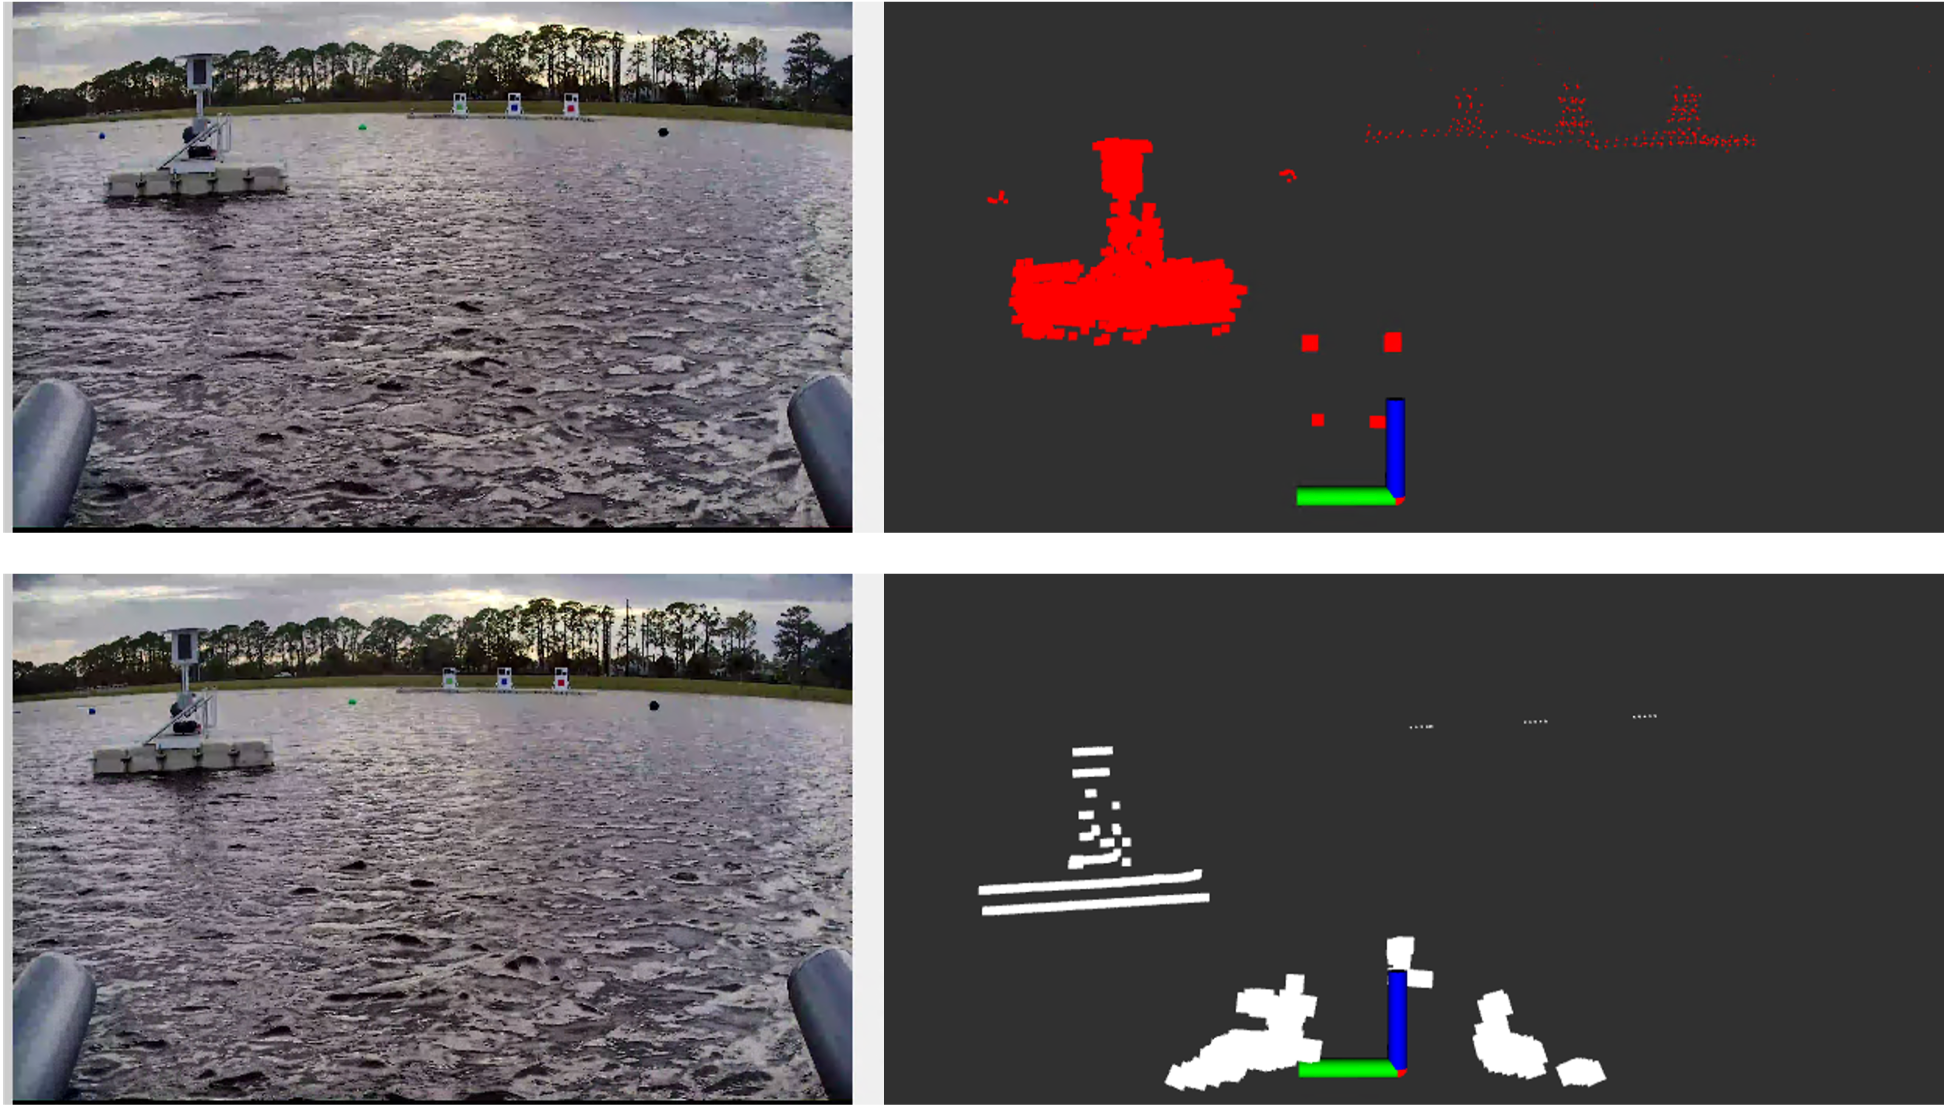
\includegraphics[width=0.8\textwidth]{Images/LiDAR_compare.png}
\caption{\textcolor{red}{place-holder image - A visual comparison of the 360 degree scan pattern of the Velodyne units (left) and the forward-scanning pattern of the Livox units (right)} }
\label{fig:lidar_scan_compare}
\end{figure}

% The superior point density of the overlapping forward-scanning  LiDAR is critical for the real-time object detection method that is discussed in \textcolor{red}{Section \#}.
% The overlapping forward-scanning LiDAR provides the spatial density required for the real-time object-detection framework described in Section \ref{gbcache}.
% For this reason, the research presented in this work exclusively utilizes LiDAR data from the Livox Horizon sensors.

Consequently, the research presented in this work relies exclusively on LiDAR data from the forward-scanning Livox Horizon sensors, whose concentrated and non-repetitive coverage provides the spatial resolution required for the real-time object-detection framework described in Section \ref{gbcache}.
        %%%%%%%%%%%%%%%%%%%%%%%%%%%%%%%%%%%%%%%%%%%%%%%%%%%%%%%%%%%%
\subsubsection{Livox Horizon} \label{sensors_livox}

% Each Livox Horizon employs two orthogonal mirrors operating at different frequencies to trace a complex Lissajous-like path that progressively fills the $81.7 \times 25.1$-degree (horizontal × vertical) \ac{FOV}, as illustrated in Figure~\ref{fig:livox_scan_pattern}. 
% The three Livox units are mounted with 40 degrees of horizontal separation, overlapping each other \ac{FOV} by $\approx 50\%$, making the system robust to failure of any single unit, as well as effectively doubling the rate of sampled points and distributing them more evenly across the center device's \ac{FOV}. 
Each Livox Horizon uses dual orthogonal mirrors oscillating at slightly different frequencies to generate a non-repetitive Lissajous-like scan pattern over its $81.7 \times 25.1$ degree \ac{FOV}. 
Overlapping these sensors by roughly $50 \%$ effectively doubles the point density along the center-line path under nominal operation, and maintains coverage under single-unit failure.
Table~\ref{table:livox_horizon_specs} presents detailed hardware specifications for the Livox Horizon.

% The rosette scan pattern is provided in \ref{fig:livox_scan_pattern}, and table \ref{table:livox_horizon_specs} presents the Livox Horizon specifications.


 
\begin{figure}[htbp]
\centering
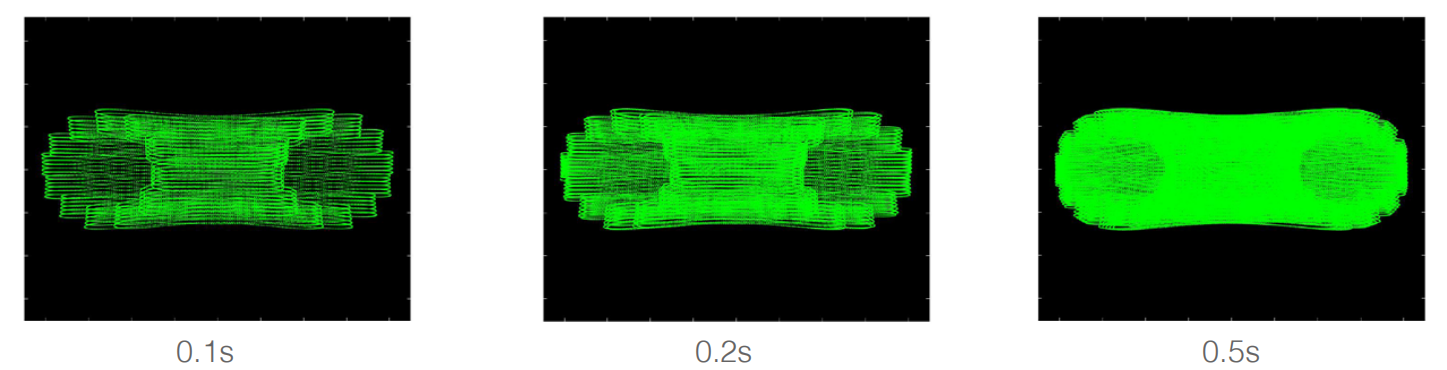
\includegraphics[width=0.8\textwidth]{Images/Livox_1.png}
\caption{Livox Horizon non-repetitive rosette scan pattern demonstrating point cloud density distribution from 0.1 to 0.5 seconds.\textcolor{red}{provide img reference}}
\label{fig:livox_scan_pattern}
\end{figure}

\begin{table}[htpb]
\centering
\caption{LiDAR Specifications}
\begin{tabular}{ll}
\hline
\multicolumn{2}{c}{Livox Horizon}\\
\hline
% \textbf{Parameter} & \textbf{Value} \\
\hline
Model & Livox Horizon \\
Horizontal Field of View & 81.7 degree \\
Vertical Field of View & 25.1 degree \\
Range & 260 m @ 80\% reflectivity \\
Point Rate (Single Return) & 240,000 pts/sec \\
Point Rate (Dual Return) & 480,000 pts/sec \\
Range Precision & ±2 cm \\
Wavelength & 905 nm \\
Scan Pattern & Non-repetitive rosette \\
Interface & Ethernet \\
Operating Frequency & 100 Hz \\
\hline
\end{tabular}
\label{table:livox_horizon_specs}
\end{table}

Each device is capable of returning up to $4.8 \times 10^5$ \ac{pps} in dual return mode, with each return consisting of position coordinates (x, y, z), target reflectivity, and timestamp.
This operational mode returns two data points for each laser emission and is useful for situations where the sensor scans semi-permeable objects such as windows, thick tree canopies, or water.
% Instead, each device is operated in single-return mode for two reasons.
% The first is a consideration of available network bandwidth.
Each sensor operates in single-return mode, primarily to reduce network load.
A conservative estimate of 16 bytes per point results in $\approx 23 \text{ Mbps}$ and would quickly overwhelm the \acp{USV} network.
% Luckily, the 905 nm near-infrared wavelength of the emitted laser experiences strong absorption by water. 
The $905 nm$ near-infrared emission is strongly absorbed by water, effectively suppressing subsurface returns.
This means that only points that are reflected by the water surface are returned with an intensity greater than zero, making it easier to filter out points in the ground plane.


%%%%%%% move to sensor calibration %%%%%%%%%%%
% Accurate fusion of data from multiple \ac{LiDAR} units requires precise knowledge of sensor geometric relationships.
% The Livox Horizon units feature onboard storage for extrinsic calibration parameters, enabling each sensor to transform its measurements to a common reference frame before transmission.
% These parameters are written to non-volatile memory on each Livox unit and applied before data transmission so that all LiDAR returns are received in the center \ac{LiDAR}'s reference frame, reducing the necessary calculation further down the data pipeline.
% \textcolor{red}{cite Livox documentation?}.
% enhancing their real-time operational advantage by reducing additional computation later in the pipeline.
% The calibration methodology to determine these extrinsic values is detailed in Section~\ref{lidar_extrinsic}.
%%%%%%%%%%%%%%%%%%%%%%%%%%%%%%%%%%%%%%%%%%%%%%%

% The 905 nm near-infrared wavelength experiences strong absorption by water, resulting in minimal returns from water surfaces.
% This characteristic benefits maritime object detection by reducing clutter from waves that would otherwise trigger false positives in clustering algorithms.

% The fundamental distinction between the Livox Horizon and traditional spinning \ac{LiDAR} lies in the scan pattern.
% A mechanically spinning sensor with N lasers produces N discrete horizontal rings that repeat identically each rotation.
% For vessels moving at typical speeds (2-5 m/s), platform displacement between rotations remains small relative to object size, resulting in near-perfect overlap of consecutive scans.
% The Livox operates differently, employing a two-dimensional scanning mechanism that traces a non-repetitive rosette pattern across the \ac{FOV}.
% Two orthogonal mirrors operating at slightly different frequencies cause the laser beam to trace a complex Lissajous-like path that progressively fills the \ac{FOV} without repetition \cite{thompson2023}.

% Scan pattern coverage accumulates over time, with longer integration periods yielding denser spatial sampling.
% At the standard 100 Hz output rate, each \ac{UDP} message contains approximately 10 milliseconds of returns.
% Over a one-second aggregation period, the rosette pattern provides substantially higher spatial coverage than a spinning sensor's fixed ring geometry.

% The non-repetitive forward-scanning nature of the Livox units means that point cloud density is not uniform across the \ac{FOV}.
% The 81.7-degree horizontal \ac{FOV} allows for overlap between the three units, achieving more uniform density across the 165-degree \ac{FOV}, matching the 4K FLIR camera coverage.

% Insert figure showing Livox scan pattern here
% \begin{figure}[htbp]
% \centering
% 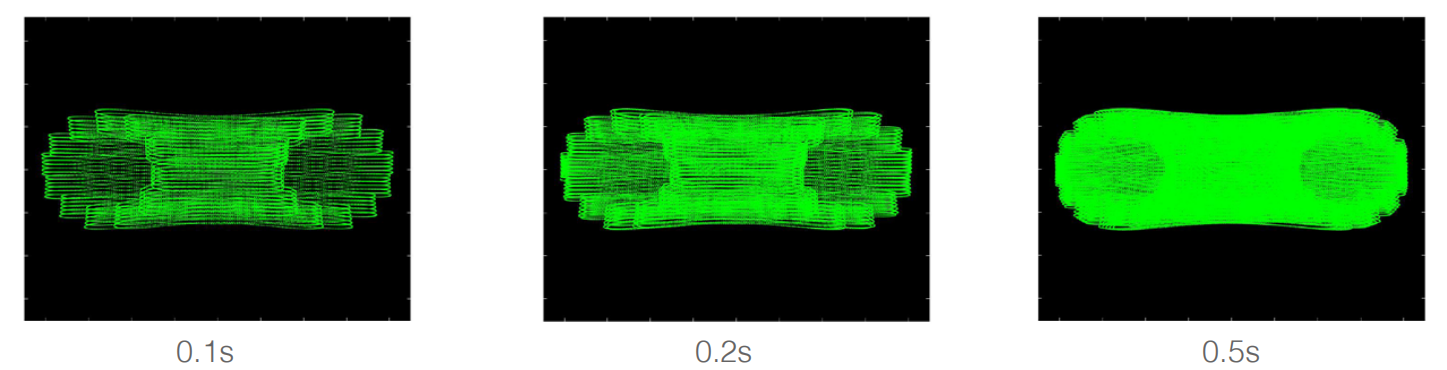
\includegraphics[width=0.8\textwidth]{Images/Livox_1.png}
% \caption{Livox Horizon non-repetitive rosette scan pattern demonstrating point cloud density distribution from 0.1 to 0.5 seconds.}
% \label{fig:livox_scan_pattern}
% \end{figure}




% A Velodyne VLP-16 in dual-return mode produces approximately 1.4 million \ac{pps} distributed across the full 360-degree plane.
% The camera \ac{FOV} encompasses approximately 165 degrees, yielding an effective point rate in the region of interest of:

% $$\text{Effective HDL-32E rate} = 1.4 \times 10^6 \times \frac{165 degree}{360 degree} \approx 641,000 \text{ pts/sec}$$

% Three Livox Horizon units in dual-return mode together produce:

% $$\text{Combined Livox rate} = 3 \times 480,000 = 1.44 \times 10^6 \text{ pts/sec}$$

% This represents a 2.25× increase in point returns within the camera view, excluding additional benefits from superior vertical sampling achieved through the non-repetitive pattern compared to fixed 32-ring geometry \cite{thompson2023}.

%%%%%%%%%%%%%%%%%%%%%%%%%%%%%%%%%%%%%%%%%%%%%%%%%%%%%%%%%%%%%%%%%%%%
\subsection{Visible Spectrum Cameras} \label{visual_cameras}

% \textcolor{red}{Expand this entire discussion}
% The visible spectrum camera suite on the Minion platform is designed to balance two factors that are particularly important for maritime perception: imaging resolution and dynamic range.
The visible-spectrum cameras housed in the camera enclosure are designed to balance image resolution and dynamic range, two critical factors for maritime perception.
A brief discussion of both of these metrics is presented here as a means to illuminate the decision to only utilize data acquired from the \ac{HDR} camera for the research in this study.

Camera resolution determines the ability to resolve small targets at a distance.
% , and appropriate imaging sensors and lenses can be selected by determining the maximum distance and minimum size at which objects need to be resolved.
% Camera resolution dictates the minimum discernible target size at range; lens and sensor parameters are therefore chosen to meet specified detection distances.
% Camera resolution governs the minimum resolvable target size; lens and sensor parameters are thus selected to ensure detection at required ranges.
To ensure adequate perception across the operational envelope, cameras must resolve objects to a required minimum resolution when the object is at the maximum detection range.  
% The resolution of an object in the image frame can be determined if the object's width $\mathit{l}$ and distance from the camera $d$ are knownwith
The relationship between an objects physical width $\mathit{l}$ and pixel width within an image $\mathit{l}_{\text{px}}$ is given by
% Provided a maximum detection range $d$ and the width of the smallest object to be detected $W$, the camera's focal length and resolution requirements can be determined by assuming a pinhole-camera model \cite{matlab_calibration}, can be derived as:
% we can determine the necessary optical focal length and resolution for the sensor.
% For an object of physical width $W$ at distance $d$, its width in the image frame $w_{\text{px}}$ is approximated by

\begin{equation}
\mathit{l}_{\text{px}} = f \; \frac{N_x}{S_w}\frac{\mathit{l}}{d}
\end{equation}

% where $\mathit{l}_{\text{px}}$ is the pixel width of an object in the image frame, 
where $f$ is the \ac{EFL} of the camera and lens, $N_x$ is the horizontal image resolution in pixels, and $S_w$ is the width of the image sensor.
% This equation is used for sensor selection by determining the minimum resolution required for the smallest object to be detected at the maximum detection range.
This equation can be used to determine camera requirements if the true size of the imaged objects are known, or to determine a reasonable expectation of object resolution if the camera values are known.
This relationship is also critical for determining the unique distortion present in every camera/lens system, detailed further in section~\ref{HDR_intrinsic}.


% Given that the smallest object we wish to detect is $0.3683$ meters wide at a distance of 60 meters, the \textcolor{red}{Insert equations for camera here}.\textcolor{blue}{The cameras in our system meet this requirement}; the object detection method used will impose a secondary constraint.
  % \begin{equation}
  % w_{\text{px}} = \frac{f \, N_x}{S_w}\frac{(0.3683)}{60}
  % % \frac{S_w}{f} = \frac{W}{d}\frac{N_x}{w_{px}}
  % \end{equation}


Defining the requirement for the minimum resolution of an object in the image frame requires an understanding of the object detection method used with visual cameras, as well as the objects being detected, both of which will be discussed in greater detail in sections ~\ref{yolo} and ~\ref{dataset}, respectively.
% For now, it is sufficient to know that the smallest object we wish to detect is $0.3683$ meters wide at a distance of 60 meters.
% , and that we have optical and digital resolution requirements to consider.
This image detection architecture scales each image frame down to a resolution of $640 \times 640$ pixels for processing efficiency, and must be considered when defining the minimum pixel density of a camera's sensor.
% This means that an image captured at $4000 \times 3000$ pixels is reduced to $650 \times 487$ pixels, which is $16.25\%$ of its original size.
% As an example, if the text on waterway signage 60 meters away is legible at a resolution of 100 pixels wide in a 1,000 $\times$ 1,000 pixel image, it would need a resolution of 162 pixels to meet the additional requirements imposed by the image detection algorithm.
Each camera within the enclosure was selected using these metrics, and object information based on the obstacles commonly associated with the RobotX Maritime Challenge in addition to other contemporaneous research \cite{thompson2023} \textcolor{red}{(check scholarly commons)}.

% Insert equation to get the horizontal focal length / horizontal resolution ratio needed for camera selection based upon the equation and information provided above
% Assuming our camera will have a landscape aspect ratio, our equation becomes 
% Since the detection network downsamples each input frame to a maximum dimension of 640 pixels while preserving aspect ratio, a landscape-oriented image with native resolution $N_x \times N_y$ (where $N_x > N_y$) is scaled such that the horizontal dimension becomes 640 pixels.
% For an object that must occupy at least $w_{\text{net}}$ pixels horizontally in the network input to be reliably detected, the camera system must satisfy
%   \begin{equation}
%   \frac{f}{S_w} = \frac{w_{\text{net}} \, d}{640 \, W}
%   \end{equation}
% \begin{equation}
%  w_{\text{px}} \left(\frac{650}{N_x}\right) = f \; \frac{N_x}{S_w}\frac{W}{d}
% \end{equation}

% where the ratio $f/S_w$ represents the normalized focal length of the camera-lens system.
% Substituting the minimum object dimensions ($W = 0.3683$ m, $d = 60$ m) and assuming a minimum network resolution requirement of $w_{\text{net}}$ pixels, this relationship defines the optical design space for camera selection.
% This makes our equation

% \begin{equation}
% w_{\text{px}} = \frac{f \, N_x^2 \, W}{(680)S_w \, d}
% \end{equation}



% The dynamic range of an imaging sensor refers to the range of signal intensities it can detect, and can be as critical as image resolution when selecting camera sensors.
Dynamic range describes the ratio between the brightest and darkest signal levels a camera sensor can record.
Light levels that exceed the camera sensor's range cause the image to appear white or "blown-out", while light levels that are too low will appear darker with detail being indistinguishable from noise.
% Dynamic range—the span of detectable signal intensities—is equally critical to sensor selection as spatial resolution.
\acp{USV} and \acp{AGV} routinely operate in environments where bright sky reflections and deep shadows are common, often within the same scene.
Therefore, selecting a camera with insufficient dynamic range may lead to washed-out highlights or lost detail in shadows.

Dynamic range, expressed in dB, is given by
\begin{equation}
 \text{Dynamic Range (dB)} = 20 \log{\left( \frac{N_{sat}}{N_{noise}}\right) }
\end{equation}
where $N_{sat}/N_{noise}$ is the ratio of the saturation to the minimum signal a camera sensor can detect above background noise.
% Higher dynamic range can be achieved through software by combining sequential multi-exposure images, or through a digital overlap \ac{HDR} (DOL-HDR) architecture with in-pixel dual conversion gain.
% Sequential multi-exposure \ac{HDR}, which stacks separate frames and is prone to ghosting or blurring, therefore 
% DOL-\ac{HDR} is preferred when precise synchronization of the imagery is required, such as sensor fusion.
% Because maritime environments routinely present both bright sky reflections and deep shadows in the same scene, dynamic range is as critical as resolution when selecting cameras for perception tasks. 
High-dynamic-range (HDR) imaging can be achieved in two primary ways. 
The first is sequential multi-exposure \ac{HDR}, in which multiple frames captured at different exposure settings are combined to extend the tonal range. 
While effective for static scenes, this approach introduces motion-related artifacts such as ghosting and motion-blur as the relative velocity increases between the sensor and objects within the frame.
The second method uses an in-sensor technique that reads multiple exposure levels simultaneously. 
By capturing short and long exposure data within a single frame, this method avoids the distortion of multi-exposure \ac{HDR}.

%%%%%%%%%%%%%%%%%%%%%%%%%%%%%%%%%%%%%%%%%%%%%%%%%%%%%%%%%%%%%%%%%%%%
\subsubsection{FLIR Blackfly S 4K Cameras} \label{sensors_FLIR}

% Three FLIR Blackfly S 4K visible-light cameras, arranged to provide a combined 165 degrees of forward-facing coverage through overlapping 65-degree lenses.  
Three FLIR Blackfly S 4K cameras are aligned to the port, center and starboard sight-lines described in section \ref{perception_geometry} to provide a combined 165-degree horizontal \ac{FOV}.
In addition to redundancy, this configuration avoids additional spherical distortion within the image that would be required to cover the same \ac{FOV} with fewer cameras.
% Each camera is paired with a Theia TL410P zoom lens with an \ac{EFL} of \textcolor{red}{???} and an image resolution of $4096 \times 4096$, ensuring that objects remain adequately resolved across the vessel's perception envelope.  
Each FLIR Blackfly has a resolution of 4096 $\times$ 4096 pixel resolution and is paired with a Theia TL410P zoom lens at a fixed \ac{EFL} $\approx$ 8 mm.
% This sensor dimension and \ac{EFL} exceeds the pixel density required to ensure object resolution across the operational envelope.


\begin{table}[htbp]
\centering
\caption{FLIR 4K SDR Camera Specifications}
\begin{tabular}{ll}
\hline
\multicolumn{2}{c}{FLIR 4K SDR Camera}\\
% HDR & Camera\\
\hline
% \textbf{Parameter} & \textbf{Value} \\
\hline
\multicolumn{2}{c}{Camera Sensor}\\
\hline
FLIR & Blackfly S 120S4C \\
% Image Sensor & Sony IMX490 \\
% Pixel Size & $3.0 \times 3.0 \mu m$ \\
Horizontal Resolution & 4000 pixels \\
Vertical Resolution & 3000 pixels \\
Aspect Ratio & 1.33:1 \\
Maximum Frame Rate & 31 fps \\
Dynamic Range & 69.4 dB \\
\multicolumn{2}{c}{Camera Lens}\\
\hline
Theia & TL410P\\
% Aperture F/\# & $2.0$ \\
Horizontal \Ac{FOV} & 65-degrees\\
Lens \Ac{EFL} & approx. 8 mm\\
% Vertical Field of View & 37 degrees \\
\hline
\end{tabular}
\label{table:SDR_camera_specs}
\end{table}

The Blackfly S sensor captures video at 31 \ac{FPS} and achieves a dynamic range of 69.4 dB, which is within the \ac{SDR}.
% This corresponds to a span of a few thousand-to-one between the darkest detectable signal and the brightest non-saturating signal.  
% The cameras capture 31 \ac{FPS} at a resolution of 4096 $\times$ 2160 pixels.
% \textcolor{red}{Add discussion of pixel density sensor selection in the context of the requirement to resolve specific objects at a minimum resolution at a maximum specific distance. This will require equations.}

%%%%%%%%%%%%%%%%%%%%%%%%%%%%%%%%%%%%%%%%%%%%%%%%%%%%%%%%%%%%%%%%%%%%
\subsubsection{Leopard Imaging HDR Camera} \label{sensors_HDR}

% A Leopard Imaging LI-USB30-IMX490-GW5400-GMSL2-065H camera, based on Sony’s IMX490 automotive-grade \ac{HDR} sensor, provides 65-degree of forward \ac{FOV}.  
The Leopard Imaging camera provides a 65-degree forward \ac{FOV} using Sony’s automotive-grade IMX490 sensor with 120 dB of dynamic range.
The \ac{HDR} is achieved via Sony’s \ac{DOL-HDR} architecture, which employs in-pixel dual-conversion gain to capture multiple exposures within a single frame period.

Table \ref{table:hdr_camera_specs} provides detailed specifications for the HDR camera, which delivers a resolution of $2880 \times 1860$ pixels at 25 frames per second with a dynamic range of 120~dB.%, extending the span of detectable light intensity to nearly one million-to-one.  

% The IMX490 accomplishes this \ac{HDR} using a digital overlap \ac{HDR} (DOL-HDR) architecture with in-pixel dual conversion gain.  

% This method captures multiple effective exposures within a single frame period, producing simultaneous multi-gain readouts from the same scene.  
This architecture produces simultaneous multi-gain readouts without sequential stacking, eliminating motion artifacts and enabling precise temporal alignment for sensor fusion.

\begin{table}[htpb]
\centering
\caption{Leopard Imaging HDR Camera Specifications}
\begin{tabular}{ll}
\hline
\multicolumn{2}{c}{Leopard Imaging HDR Camera}\\
% HDR & Camera\\
\hline
% \textbf{Parameter} & \textbf{Value} \\
\hline
% Make & Leopard Imaging \\
Leopard Imaging & LI-IMX490-GW5400-GMSL2-065H \\
Image Sensor & Sony IMX490 \\
Pixel Size & 3.0 $\times$ 3.0 $\mu$m \\
Horizontal Resolution & 2880 pixels \\
Vertical Resolution & 1860 pixels \\
Aspect Ratio & 1.55:1 \\
Maximum Frame Rate & 25 fps \\
Dynamic Range & 120 dB \\
Lens \Ac{EFL} & 7.9 mm\\
Aperture F/\# & $2.0$ \\
\Ac{FOV} & 65-degrees (H), 37-degrees (V) \\
% Vertical Field of View & 37 degrees \\
\hline
\end{tabular}
\label{table:hdr_camera_specs}
\end{table}


% This performance is enabled by a digital overlap \ac{HDR} (DOL-HDR) architecture with in-pixel dual conversion gain.  
% By capturing multiple gain levels within a single frame period, the sensor produces simultaneous multi-gain readouts without relying on sequential multi-exposure stacking.  
% This design eliminates ghosting and motion artifacts, which are common when either the platform or surrounding targets move between exposures.  

% \subsubsection{Leopard Imaging HDR Camera}

% To overcome these limitations, a \ac{HDR} camera from Leopard Imaging was integrated, based on Sony’s IMX490 automotive-grade \ac{HDR} sensor.  
% This camera provides 65 degrees of forward coverage and achieves approximately 120~dB of dynamic range, enabling preservation of fine image details across extreme lighting conditions, including bright sky, reflective water, and shaded objects.  



% This substantial increase in dynamic range, combined with robust performance under challenging illumination, made the IMX490-based \ac{HDR} camera the primary visual spectrum sensor for \ac{LiDAR}-camera fusion research in this dissertation.  
% Preliminary results from a comparative study by Liebergall et al.~\cite{liebergall} further supported this decision, showing improved detection consistency with the \ac{HDR} sensor compared to the FLIR 4K cameras.  
% Although later published results did not fully corroborate the preliminary findings, those results became available only after the dataset for this research had been collected.  
% Accordingly, the IMX490 \ac{HDR} camera served as the main forward-facing visual spectrum sensor throughout this study.  



% The 2880×1860 resolution provides sufficient spatial detail for detecting objects at relevant ranges in autonomous vessel navigation, while the 25 fps frame rate adequately supports typical vessel speeds and maneuvering.

% The IMX490's native \ac{HDR} combines multiple exposures in a single frame period, achieving 120 dB dynamic range without sequential multi-exposure capture.
% This simultaneous approach eliminates motion artifacts associated with temporal bracketing, which is critical when both the platform and targets are in motion.
% Image quality validation and intrinsic calibration are addressed in Section 3.2.1.1, including lens distortion characterization and camera matrix estimation.
% The combination of wide dynamic range, moderate resolution, and calibrated geometry provides the image quality necessary for training and evaluating vision-based detection models in Chapter 5.

% Thompson et al. \cite{thompson2023} originally developed this camera hardware and integration approach, establishing a foundation for maritime perception research.
% The primary enhancement introduced in this work comprises in-band timestamp embedding and temporal drift correction, detailed in Section 3.2.2, which are essential for rigorous multi-modal sensor fusion analysis.

%%%%%%%%%%%%%%%%%%%%%%%%%%%%%%%%%%%%%%%%%%%%%%%%%%%%%%%%%%%%%%%%%%%%
\subsubsection{Camera Selection} \label{camera_selection}

The combination of image resolution and \ac{EFL} of both cameras  exceeds the pixel density required to ensure object resolution across the operational envelope.
FLIR Blackfly S 4K cameras exceed the resolution requirements, but their limited dynamic range of 69.4~dB makes them prone to over-exposure and reduced contrast under extreme lighting conditions. 
% They support an effective dynamic range of 69.4~dB, which corresponds to a span of just a few thousand-to-one between the darkest detectable signal and the brightest non-saturating signal. 
% As a result, the cameras are prone to over-exposure in high-brightness maritime conditions, particularly when imaging reflective water surfaces or bright sky backgrounds, leading to loss of highlight detail and reduced contrast. 

\begin{figure}[htbp]
\centering
\makebox[\textwidth][c]{%
    \begin{subfigure}[t]{0.35\textwidth}
        \centering
        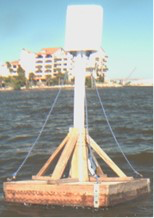
\includegraphics[width=\textwidth]{Images/SDR_bright.png}
        \caption{SDR visual camera (5 MP)}
        \label{fig:fov_cam}
    \end{subfigure}
    \hspace{2em} % horizontal spacing between them
    \begin{subfigure}[t]{0.378\textwidth}
        \centering
        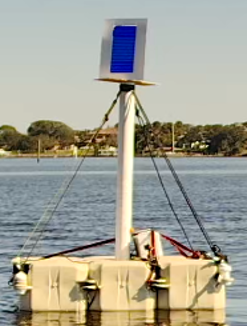
\includegraphics[width=\textwidth]{Images/HDR_bright.png}
        \caption{HDR visual camera (5 MP)}
        \label{fig:fov_lidar}
    \end{subfigure}%
}
\caption{\textcolor{red}{place-holder image – A visual comparison of the \ac{SDR} FLIR 4k camera (left) and the \ac{HDR} Leopard Imaging camera (right) in low-light conditions.}}
\label{fig:HDR_compare}
\end{figure}

In contrast, the Leopard Imaging \ac{HDR} camera offers slightly lower image resolution at a comparable effective focal length but provides substantially greater dynamic range.
% enabling detail preservation across bright and shaded regions within the same frame.  
This wider dynamic range enables more consistent color fidelity and image contrast under suboptimal lighting conditions, as illustrated in Figure~\ref{fig:HDR_compare}.

% Many tasks in the 2024 Maritime RobotX Challenge required \acp{USV} to accurately distinguish object colors as part of their operational decision-making.
This capability motivated in the selection of the \ac{HDR} camera as Minion's primary visual camera sensor for the 2024 Maritime RobotX Challenge, included several tasks required \acp{USV} to acuratly identify object colors to make operational decisions.
A comparitive study by Liebergall et al.~\cite{liebergall} further supported this decision, as preliminary results indicated improved object detection results with data from the \ac{HDR} over the FLIR \ac{SDR} camera. 
Because the data collected during that competition formed the foundation of this dissertation, the Leopard Imaging \ac{HDR} camera the primary visual spectrum sensor was selected for all research presented in this paper.

% For these reasons, the \ac{HDR} camera was designated as the primary forward-facing visual spectrum sensor for the \ac{LiDAR}-camera fusion research presented in this paper.  




%%%%%%%%%%%%%%%%%%%%%%%%%%%%%%%%%%%%%%%%%%%%%%%%%%%%%%%%%%%%%%%%%%%%
%%%%%%%%%%%%%%%%%%%%%%%%%%%%%%%%%%%%%%%%%%%%%%%%%%%%%%%%%%%%%%%%%%%%

\subsection{PinPoint GPS/INS} \label{sensors_GPS}

The Minion platform features a PinPoint \ac{GPS}/\ac{INS} equipped with dual-antennae for orientation and differential corrections for millimeter precision geolocation.
The sensor performs two critical functions for the \ac{USV}: tracking vessel position and orientation and precise global time for sensor synchronization.
The \ac{GPS} receiver functions as the master clock for the entire synchronization hierarchy described in Section 3.2.2.1, while the integrated \ac{IMU} enables high-rate pose updates between \ac{GPS} fixes.

% Global Navigation Satellite System signals inherently carry highly accurate timing information, as satellite positioning operates through precise measurement of signal delay from multiple satellites with synchronized atomic clocks.
% The PinPoint receiver extracts this timing information and distributes it over the vessel's network using Network Time Protocol.
% The \ac{GPS} unit was assigned a static IP address of 201.7.90.30 on the Minion network and configured to broadcast \ac{GPS}-disciplined time via Network Time Protocol.
% The Atlas PC main computer synchronizes its clock to this \ac{GPS} source with typical accuracy in the tens to hundreds of nanoseconds, limited primarily by network latency rather than \ac{GPS} accuracy.

% This \ac{GPS} time reference propagates through the synchronization hierarchy to every computing resource on the platform.
% Atlas functions as a Network Time Protocol server for the NVIDIA Jetson Xavier camera computer, which subsequently operates as a Precision Time Protocol master for the Livox Horizon \ac{LiDAR} sensors.
% This cascaded approach ensures timestamps from all sensors—cameras, \ac{LiDAR}, and \ac{GPS}/\ac{IMU}—share a common time reference traceable to \ac{GPS} time.

% Beyond timekeeping, the \ac{GPS}/\ac{IMU} system continuously tracks platform position and orientation, which is required for \ac{LiDAR} temporal aggregation.
% As described in Section 3.1.1.3, accumulating \ac{LiDAR} points over several seconds necessitates compensation for vessel motion during that period.
% The PinPoint system fuses \ac{GPS} position measurements with \ac{IMU} acceleration and rotation data through an Extended Kalman Filter to produce pose estimates at rates substantially higher than \ac{GPS} alone could provide.
% \ac{GPS} fixes arrive at 1-10 Hz depending on satellite visibility, while the \ac{IMU} operates at hundreds of hertz.
% The fusion algorithm propagates pose estimates forward using \ac{IMU} integration between \ac{GPS} updates, subsequently correcting accumulated drift when new \ac{GPS} measurements arrive.

% The resulting pose solution provides six-degree-of-freedom state estimates—three-dimensional position and three-dimensional orientation—at sufficient temporal resolution to interpolate platform pose to the exact timestamp of each \ac{LiDAR} point.
% This capability supports the transformation methodology presented in Chapter 5, where \ac{LiDAR} points acquired at different times during motion are transformed to a common reference frame before projection onto camera images.

% The PinPoint \ac{GPS}/\ac{IMU} connects to the Minion computing infrastructure via Ethernet, utilizing both Network Time Protocol for time distribution and User Datagram Protocol for pose data transmission.
% \ac{ROS} driver nodes on the Atlas PC receive and parse the binary \ac{GPS}/\ac{IMU} messages, publishing pose estimates as standard \ac{ROS} geometry messages.
% These messages incorporate position (latitude, longitude, altitude), orientation (roll, pitch, yaw), uncertainty estimates, and \ac{GPS} fix quality flags.
% The \ac{ROS} tf2 library consumes these pose estimates to maintain the time-varying transformation tree relating sensor frames to platform and world frames, enabling automated coordinate transformation for sensor fusion.

% The \ac{GPS}/\ac{IMU} defines the local reference frame for the platform \texttt{base\_link}, with position expressed in geographic coordinates (WGS84 datum) and orientation relative to true north and local gravity.
% This world-referenced system serves as the common reference for transforming observations from multiple sensors acquired at different times during motion.
% Transformation from sensor-local frames to the \ac{GPS}/\ac{IMU} world frame requires knowledge of sensor-to-platform extrinsic calibration parameters.
% These parameters are determined through calibration procedures described in Section 3.2.1.2 for cameras and Section 3.2.1.3 for \ac{LiDAR} sensors.
% With extrinsic parameters established, the \ac{GPS}/\ac{IMU} pose solution enables transformation of any sensor observation to world coordinates or to any other sensor's reference frame.

% Maritime environments present challenges for \ac{GPS}/\ac{IMU} systems that differ from land vehicle applications.
% Water surface reflections induce multipath interference in \ac{GPS} signals, while vessel pitch and roll motion exercises the full range of the \ac{IMU}.
% The PinPoint system was designed for marine applications and incorporates algorithms to address these factors while maintaining accuracy during vessel maneuvering.
% \ac{GPS} accuracy degrades in areas with limited satellite visibility, such as proximity to tall structures, bridges, or fjord-like coastal terrain.
% The \ac{IMU} provides short-term pose continuity during \ac{GPS} outages, though accumulated drift limits the duration for which pure inertial navigation remains accurate.
% Data collection operations were conducted in open water with favorable satellite visibility, ensuring consistent \ac{GPS} fix quality throughout recording sessions.

% The \ac{GPS}/\ac{IMU} system enables two functions essential for multi-modal sensor fusion research.
% First, \ac{GPS}-disciplined time distributed to all sensors ensures timestamps from cameras, \ac{LiDAR}, and \ac{GPS} itself reference the same time base, providing frame-accurate temporal association across modalities.
% Second, continuous pose estimates enable transformation of temporally distributed observations to common reference frames, supporting \ac{LiDAR} aggregation during motion and registration of sensor fields of view for fusion operations.
% Combined with the synchronization verification and drift correction procedures described in Section 3.2.2, these capabilities establish the temporal and spatial foundation for rigorous object detection performance evaluation across sensing modalities.
% The \ac{GPS}/\ac{IMU} thus functions not merely as a navigation sensor but as critical infrastructure enabling the multi-modal perception analysis central to this research.

%%%%%%%%%%%%%%%%%%%%%%%%%%%%%%%%%%%%%%%%%%%%%%%%%%%%%%%%%%%%%%%%%%%%
%%%%%%%%%%%%%%%%%%%%%%%%%%%%%%%%%%%%%%%%%%%%%%%%%%%%%%%%%%%%%%%%%%%%
\section{Compute Hardware and Network} \label{sec:Atlas_LAN}

The Minion autonomous surface vessel employs a distributed computing architecture that balances real-time processing requirements with operational flexibility and redundancy. The computing infrastructure consists of high-performance workstation computers serving as the primary processing platforms, an embedded computer integrated with the camera sensors for video encoding and edge processing, and a dedicated Gigabit Ethernet local area network interconnecting all platform systems. This architecture distributes computational workloads according to sensor proximity and processing requirements while maintaining centralized coordination through the Robot Operating System middleware. The following subsections detail the hardware specifications, system architecture, and network infrastructure that enable real-time multi-modal perception for maritime object detection and sensor fusion.

%%%%%%%%%%%%%%%%%%%%%%%%%%%%%%%%%%%%%%%%%%%%%%%%%%%%%%%%%%%%%%%%%%%%
\subsection{Atlas} \label{atlas}

The primary computing infrastructure for the Minion autonomous surface vessel consists of two identical high-performance workstation computers designated Minion A and Minion B. These systems, built on the Nvidia Atlas platform, provide the computational resources necessary for real-time sensor data processing, object detection algorithm execution, and autonomous navigation decision-making. The dual-computer configuration provides operational redundancy, allowing hot-swapping between systems for software development, testing, and failover scenarios without requiring vessel downtime.

Each Atlas PC features enterprise-grade computing hardware selected to meet the demanding requirements of real-time multi-modal perception and machine learning inference. The systems incorporate multi-core processors with sufficient parallel processing capability to handle simultaneous operation of LiDAR point cloud processing, computer vision algorithms, sensor fusion, and navigation planning. Adequate RAM capacity enables loading of large deep learning models and maintenance of temporal buffers for multi-second LiDAR aggregation as described in %[[03_Livox_Horizon#Temporal Aggregation and Motion Compensation|Section 3.1.1.3]].

High-speed solid-state storage provides the throughput necessary to record multiple synchronized sensor streams to disk during data collection operations. Recording sessions simultaneously capture raw LiDAR point clouds, compressed video streams from three cameras, GPS/INS pose messages, and timestamped detection results, generating aggregate data rates that can exceed hundreds of megabytes per second. The storage subsystem must sustain these write rates for extended periods without buffer overflow or frame dropping.

The presence of two functionally equivalent Atlas PCs serves multiple operational purposes. During development and testing, one system can run experimental software while the other maintains a stable baseline configuration, enabling rapid testing iteration without compromising the ability to revert to known-good software states. For field operations, one system serves as the active primary while the other remains available as an immediate backup in case of hardware failure or software crashes.

The dual-system configuration also facilitates the ROS ecosystem transition occurring during the timeframe of this research. ROS 1 (Robot Operating System version 1), while mature and well-supported, reached end-of-life for active development, prompting migration to ROS 2 with its improved real-time performance, security features, and inter-process communication architecture. Maintaining one system on ROS 1 while transitioning the other to ROS 2 enabled gradual software migration while preserving operational capability.

**Minion A** operates Ubuntu 22.04 LTS (Long Term Support) with ROS 2 Humble Hawksbill, representing the future software direction for the platform. **Minion B** operates Ubuntu 20.04 LTS with ROS 1 Noetic Ninjemys, providing continuity with existing software packages and maintaining compatibility with legacy sensor drivers and perception algorithms developed over prior research campaigns.

The Atlas platform hosts several software subsystems essential to the perception and autonomy pipeline:

**LiDAR Processing**: The Livox ROS SDK executes on the Atlas PC, receiving UDP message streams from the three Livox Horizon sensors and publishing unified point clouds to ROS topics. Point cloud aggregation and transformation algorithms, which implement the motion compensation methodology detailed in Chapter 5, also execute on this platform.

**Vision Processing**: While H.264/H.265 video encoding occurs on the Jetson Xavier camera enclosure, the Atlas PC receives and decodes the RTSP video streams, extracting embedded SEI timestamps as described in \textcolor{red}{Section 3.2.2.2} and publishing decoded frames as ROS image messages.

**Object Detection**: The YOLOv8 vision-based object detection models and GB-CACHE LiDAR clustering algorithms both execute on the Atlas hardware, leveraging multi-core CPU resources and, where applicable, GPU acceleration for deep learning inference.

**Sensor Fusion**: Late fusion algorithms that combine detections from vision and LiDAR modalities operate on the Atlas platform, accessing synchronized sensor observations via ROS topic subscriptions and temporal alignment procedures detailed in Section 3.2.2.

**Navigation and Control**: Path planning, collision avoidance, and vessel control algorithms utilize the processed perception results to generate navigation commands, though autonomous control implementation falls outside the scope of this dissertation's focus on perception performance analysis.

%%%%%%%%%%%%%%%%%%%%%%%%%%%%%%%%%%%%%%%%%%%%%%%%%%%%%%%%%%%%%%%%%%%%
\subsection{Camera Enclosure} \label{comp:camera_enclosure}

% # Camera Enclosure Computing Platform

The camera enclosure assembly integrates six camera sensors with dedicated computing hardware housed in a weatherproof enclosure mounted on the vessel's superstructure. At the core of this assembly is an NVIDIA Jetson Xavier embedded computer, which performs real-time H.264/H.265 video encoding, manages timestamp embedding for temporal synchronization, and serves critical time distribution functions within the hierarchical clock architecture. This distributed computing approach places video processing at the camera location rather than transmitting raw uncompressed video over the network, substantially reducing bandwidth requirements while enabling sophisticated in-stream timestamp embedding.

The camera enclosure was designed to be a fully-integrated and self-contained perception platform, and was developed in tandem for the RobotX competition in 2022 and the PhD research of D. Thompson \cite{thompson2023}.

% ## NVIDIA Jetson Xavier Platform

The NVIDIA Jetson Xavier represents an embedded computing platform designed for edge AI and computer vision applications, combining ARM-based CPU cores with a powerful GPU architecture optimized for machine learning inference and media encoding. The system-on-module (SOM) design integrates processor, GPU, memory, and I/O interfaces in a compact form factor suitable for environmentally sealed enclosures.

Key specifications relevant to the camera processing application include:

% - **CPU**: 8-core ARM Carmel processor providing sufficient computational capacity for GStreamer pipeline management and network protocol handling
% - **GPU**: 512-core Volta architecture GPU with hardware-accelerated video encoding/decoding
% - **Memory**: Unified memory architecture shared between CPU and GPU, enabling efficient data exchange for media processing pipelines
% - **Video Encoding**: Dedicated hardware encoding engines capable of real-time H.264 and H.265 compression for multiple simultaneous video streams
% - **Network**: Gigabit Ethernet interface for connection to the vessel LAN described in [[03_Network|Section 3.1.2.3]]
% - **Storage**: NVMe SSD for local video recording and operating system hosting

% The Jetson Xavier is assigned IP address 201.7.90.147 on the Minion LAN, providing network addressability for NTP synchronization, video streaming, and remote administration.

% ## Video Processing Pipeline

The primary computational responsibility of the Jetson Xavier is real-time video encoding and streaming of the three HDR camera feeds. Raw video frames from the cameras enter the system via USB 3.0 UVC (Universal Video Class) interfaces, accessed through the Video for Linux (V4L2) kernel subsystem. The GStreamer multimedia framework constructs processing pipelines that capture these raw frames, apply format conversions, encode to H.264 or H.265 compressed formats, embed timestamps as Supplemental Enhancement Information (SEI) NAL units, and transmit the resulting streams via RTSP (Real-Time Streaming Protocol) over the local network.

The video encoding workflow, detailed comprehensively in \textcolor{red}{Section 3.2.2.2}, exploits the Jetson's dedicated hardware encoding engines to achieve real-time compression of three simultaneous 2880×1860 pixel video streams. Hardware encoding offloads the computationally intensive compression operations from the CPU, enabling sustainable operation without thermal throttling during extended recording sessions.

The compressed video streams are transmitted to the Atlas PC main computing platform via RTSP over UDP, where they are decoded and published as ROS image messages for consumption by object detection algorithms. This architecture distributes the encoding burden to the camera enclosure while centralizing detection processing on the more powerful Atlas hardware.

% ## Timestamp Embedding Implementation

A critical function performed by the Jetson Xavier is the embedding of precise system timestamps directly into the encoded video bitstream. As detailed in \textcolor{red}{Section 3.2.2.2},
% [[02_Video_Pipeline|Section 3.2.2.2]]
custom GStreamer pipeline elements inject SEI NAL units containing GPS-synchronized timestamps alongside encoded video frames. This in-band metadata approach ensures that timing information persists with the video data through network transmission, recording, and playback, enabling the temporal drift correction methodology described in \textcolor{red}{Section 3.2.2.3}
% [[03_Temporal_Drift|Section 3.2.2.3]].
The timestamp embedding process requires that the Jetson's system clock be accurately synchronized before video capture begins. Startup verification procedures, implemented in the camera launch scripts, confirm NTP synchronization with the Atlas PC before initiating video streaming. This verification prevents the recording of video with uncalibrated timestamps that would compromise subsequent temporal alignment operations.

% ## Network Time Protocol Client Role

Within the hierarchical time synchronization architecture detailed in \textcolor{red}{Section 3.2.2.1},
% [[01_Clock_Sync|Section 3.2.2.1]]
the Jetson Xavier operates as an NTP client receiving GPS-disciplined time from the Atlas PC, which itself synchronizes to the Pinpoint GPS receiver. The Chrony NTP daemon executes on the Jetson, periodically querying the Atlas NTP server and adjusting the local system clock to maintain alignment with GPS time.

NTP provides synchronization accuracy on the order of milliseconds over local network connections, which proves sufficient for the video frame timestamps given the 10 frames-per-second capture rate employed during data collection (100 milliseconds between frames). For reference, preliminary analysis documented in technical summaries measured average end-to-end video latency of approximately 127 milliseconds with no dropped or repeated frames, demonstrating adequate temporal stability.

The startup verification scripts check two conditions before launching video encoding:

% 1. **Chrony synchronization status**: Verification that the NTP daemon has established contact with the upstream Atlas NTP server and completed initial clock adjustment
% 2. **System time validity**: Confirmation that the system clock reflects plausible GPS time rather than a default epoch time indicating loss of synchronization

These checks ensure that video timestamps derive from GPS-disciplined time from the moment recording begins.

% ## Precision Time Protocol Master Role

Beyond serving as an NTP client, the Jetson Xavier operates as a Precision Time Protocol (PTP) master clock providing sub-microsecond synchronization to the three Livox Horizon LiDAR sensors. The IEEE 1588 PTP implementation, provided by the \texttt{ptp4l} daemon from the Linux PTP project, transmits periodic timing packets over the Ethernet network carrying hardware-timestamped synchronization messages.
PTP achieves substantially higher timing accuracy than NTP—on the order of microseconds rather than milliseconds—by exploiting hardware timestamping capabilities in network interfaces and accounting for symmetric network propagation delays. This precision proves essential for LiDAR applications where individual laser returns must be timestamped with sub-millisecond accuracy to enable precise spatial reconstruction during vehicle motion.

The Livox sensors discover and synchronize to the PTP master automatically via the Best Master Clock Algorithm (BMCA), which evaluates available PTP sources on the network and selects the optimal time reference. In the Minion configuration, the Jetson Xavier represents the only PTP master on the camera enclosure network segment, ensuring unambiguous selection by the LiDAR units.

Verification of PTP synchronization is performed using the Livox Viewer software application, which connects to each LiDAR unit and displays synchronization status indicators. Proper operation is confirmed by the presence of "1588 signal detected" status and active time synchronization indicators on all three Livox devices. This verification occurs as part of system startup procedures before data collection operations.

% ## Physical Integration and Environmental Protection

The camera enclosure assembly provides environmental protection for the computing hardware and camera sensors in the maritime operating environment. The weatherproof housing protects against salt spray, rain, and humidity while providing thermal management for the Jetson Xavier and associated electronics. The physical integration effort, originally performed by \cite{thompson2023}, positioned the three cameras to achieve the \ac{FOV} geometry described in \textcolor{red}{Section 3.1.1.1}
% [[01_Perception_Geometry|Section 3.1.1.1]] 
while maintaining manageable cable runs to the central computing enclosure.

Power distribution within the enclosure provides regulated voltage to the Jetson Xavier, the three cameras, and network equipment. The assembly includes a Power-over-Ethernet (PoE) switch if required for LiDAR power delivery, though the specific power architecture depends on the configuration of the three Livox Horizon units and their placement relative to the camera enclosure.

% ## Local Recording Capability

While the primary video data path streams compressed video to the Atlas PC for ROS recording, the Jetson Xavier possesses local recording capability via its NVMe solid-state storage. This redundancy provides backup recording in case of network disruptions or Atlas PC failures, ensuring that video data can be recovered even if the primary data path fails during a recording session.

Local recording can also serve diagnostic purposes, enabling comparison of locally-saved video files with network-transmitted ROS bag data to validate timestamp accuracy and detect any frame dropping or duplication during network transmission. The temporal drift analysis methodology described in \textcolor{red}{Section 3.2.2.3}
% [[03_Temporal_Drift|Section 3.2.2.3]] 
exploits this local recording capability by comparing locally-saved video frames with network-transmitted ROS messages to quantify systematic timing offsets introduced by the encoding-transmission-decoding pipeline.

% ## Integration Summary

The camera enclosure computing platform, centered on the NVIDIA Jetson Xavier embedded computer, provides several essential functions:

% - Real-time hardware-accelerated video encoding for three simultaneous HDR camera streams
% - Timestamp embedding via SEI NAL unit injection to preserve temporal synchronization information
% - NTP client synchronization to GPS-disciplined time distributed from the Atlas PC
% - PTP master clock services for sub-microsecond LiDAR temporal alignment
% - Weatherproof physical integration of cameras and computing hardware
% - Backup local recording capability for data redundancy

The distributed computing architecture, which places video encoding at the camera location while performing object detection and fusion on the Atlas PC, optimizes network bandwidth utilization while maintaining frame-accurate temporal synchronization through the hierarchical GPS-NTP-PTP clock distribution system. This infrastructure provides the foundation for the multi-modal perception analysis central to this research, enabling simultaneous capture of temporally-aligned camera and LiDAR observations as detailed in Chapter 5.

%%%%%%%%%%%%%%%%%%%%%%%%%%%%%%%%%%%%%%%%%%%%%%%%%%%%%%%%%%%%%%%%%%%%
\subsection{Network Structure} \label{comp:network}

% # Network Infrastructure

The Minion autonomous surface vessel employs a dedicated Gigabit Ethernet local area network (LAN) to interconnect computing platforms, sensors, and navigation equipment. This network serves multiple critical functions: sensor data transmission, time synchronization protocol distribution, remote administration access, and inter-process communication for the Robot Operating System (ROS) middleware. The network architecture prioritizes reliability and deterministic latency to support real-time perception and control operations in the challenging maritime environment.

% ## Network Topology and Addressing

The vessel LAN operates on the 201.7.90.0/24 private subnet, providing 254 usable host addresses for platform devices. Static IP address assignment ensures predictable network routing and simplifies configuration of time synchronization services, which require knowledge of specific server addresses. 

Key platform components are assigned the following static IP addresses:

% | Device                         | IP Address        | Function                               |
% | ------------------------------ | ----------------- | -------------------------------------- |
% | Pinpoint GPS/INS               | 201.7.90.30       | GPS-disciplined NTP time source        |
% | Atlas PC (Minion A/B)          | 201.7.90.43:17/18 | Main computing, NTP server, ROS core   |
% | Jetson Xavier Camera Enclosure | 201.7.90.147      | Video encoding, NTP client, PTP master |
% | Livox Horizon LiDAR Units (3x) | 201.7.90.43:45    | Point cloud data via UDP, PTP clients  |

The static addressing scheme facilitates configuration of the hierarchical time synchronization architecture described in \textcolor{red}{Section 3.2.2.1}
% [[01_Clock_Sync|Section 3.2.2.1]], 
where the Pinpoint GPS at 201.7.90.30 serves as the NTP root, the Atlas PC operates as an NTP server for downstream clients, and the Jetson Xavier at 201.7.90.147 functions as both an NTP client and PTP master clock.

% ## Physical Network Infrastructure

The LAN physical layer employs Cat5 Ethernet cabling supporting single gigabit link speeds. Ruggedized connectors and marine-grade cabling provide environmental protection against moisture, salt spray, and vibration. Cable runs between environmentally sealed enclosures utilize industrial IP67-rated connectors to maintain water ingress protection at connection points.

A central Gigabit Ethernet switch, housed in the main electronics enclosure alongside the Atlas PCs, provides the network backbone. This managed switch enables Quality of Service (QoS) configuration to prioritize time-critical data streams, though specific QoS policies depend on operational requirements and may prioritize either sensor data or time synchronization traffic depending on application phase.

The camera enclosure assembly includes a secondary Ethernet switch to provide network connectivity for the three Livox Horizon LiDAR units mounted on or near the camera mast. This switch connects to the main vessel switch via a single trunk line, reducing the number of cable runs between the mast and main hull while providing local switching for LiDAR and camera traffic.

% ## Data Flow Architecture

The network carries several distinct categories of traffic with varying bandwidth and latency requirements:

% **Video Streaming**: 
The three HDR cameras generate H.264/H.265 encoded video streams transmitted via Real-Time Streaming Protocol (RTSP) over UDP from the Jetson Xavier (201.7.90.147) to the Atlas PC. At 2880x1860 resolution and 5-15 frames per second with H.264 compression, the RTSP bitrate is calculated before the stream begins dependent upon the requested stream frame-rate (5-15 fps) (INSERT bitrate formula here).

% **LiDAR Point Clouds**: 
The three Livox Horizon sensors transmit point cloud data as UDP packets at 100 Hz. Each sensor operating in dual-return mode at 480,000 points/second generates approximately 15-20 Mbps of network traffic, totaling 45-60 Mbps for the three-sensor array. These UDP streams flow from the LiDAR units through the camera enclosure switch to the Atlas PC, where the Livox ROS SDK receives and publishes them to ROS topics.

% **GPS/INS Data**: 
The Pinpoint GPS/INS transmits pose solution messages via UDP at 1-10 Hz depending on configuration. These messages, containing position, velocity, and orientation estimates with associated uncertainties, require minimal bandwidth (typically <1 Mbps) but demand low latency to support real-time navigation and control.



% **ROS Inter-Process Communication**: 
The Robot Operating System middleware employs TCP/IP for initial service discovery and parameter configuration, then establishes direct peer-to-peer TCP or UDP connections for topic publish/subscribe message exchange. ROS traffic patterns depend on the specific nodes and topics active during operation, but can include republication of decoded video frames, detection results, and diagnostic messages.

% ## Network Bandwidth Utilization

Aggregate network traffic during typical data collection operations totals approximately 60-105 Mbps for sensor data (video + LiDAR) plus nominal overhead for GPS, time synchronization, and ROS messaging. This represents 6-10% utilization of the Gigabit Ethernet infrastructure, providing substantial margin for bursts, protocol overhead, and future expansion.

The network design deliberately over-provisions bandwidth relative to steady-state requirements to ensure that occasional traffic bursts such as simultaneous high-motion video frames that compress poorly, or retransmission of dropped UDP packets do not introduce congestion-induced latency. Maintaining sub-millisecond network latency proves critical for accurate NTP clock synchronization and prevents video frame jitter that would complicate temporal alignment.

% ## Reliability and Fault Tolerance

Several aspects of the network architecture address reliability concerns:

% **Redundant Atlas PCs**: 
The dual Atlas computer configuration enables network continuity if one system fails. ROS nodes can be migrated to the standby system, though operational procedures must ensure that only one system operates as the NTP server to prevent time synchronization conflicts.

**Local Recording**: Both the Jetson Xavier camera enclosure and Atlas PCs possess local storage for recording sensor data. If network connectivity fails during a data collection mission, sensors can continue recording locally for later retrieval, preventing complete data loss.

% **UDP Transport**: 
The use of connectionless UDP for high-bandwidth sensor data (video, LiDAR) avoids the head-of-line blocking and retransmission delays inherent in TCP. While UDP provides no delivery guarantee, the high-bandwidth over-provisioned network rarely experiences packet loss, and perception algorithms prove tolerant to occasional frame drops.

% **Managed Switch**: 
Network diagnostic capabilities of the managed Ethernet switch enable monitoring of port status, bandwidth utilization, and error counters. These diagnostics assist in identifying failing cables, connector corrosion, or electromagnetic interference that might degrade network performance in the marine environment.

% ## Remote Access and Administration

The vessel network includes provisions for remote access during development and testing, typically via a wireless access point or cellular router that bridges the vessel LAN to external networks. This capability enables:

% - Remote monitoring of system status and sensor data during at-sea operations
% - Software updates and configuration changes without requiring physical access to computing hardware
% - Remote debugging and log file retrieval when troubleshooting system issues
% - Off-vessel recording of ROS bag files to remote storage for dataset archival

Security considerations for remote access include firewall configuration to restrict inbound connections, authentication requirements for SSH administrative access, and potential disconnection of external network access during sensitive operations to prevent unauthorized interference.

% ## Integration with Time Synchronization Architecture

The network infrastructure provides the physical medium for the hierarchical time distribution system detailed in \textcolor{red}{Section 3.2.2.1}
% [[01_Clock_Sync|Section 3.2.2.1]]. 
The quality of clock synchronization achievable depends critically on network characteristics:

% **NTP Synchronization**: 
Network latency and jitter between the Pinpoint GPS (201.7.90.30) and Atlas PC, and between Atlas and Jetson Xavier (201.7.90.147), directly impact achievable NTP accuracy. The dedicated Gigabit infrastructure with minimal competing traffic provides sub-millisecond latency sufficient for millisecond-level NTP synchronization.

% **PTP Synchronization**: 
The IEEE 1588 Precision Time Protocol achieves sub-microsecond accuracy by exploiting hardware timestamping in network interfaces and accounting for symmetric propagation delay. The Jetson Xavier PTP master and Livox Horizon PTP clients communicate via the camera enclosure switch, benefiting from short cable runs and minimal network hops that reduce timing uncertainty.

% **Synchronization Verification**: 
The network enables remote access to synchronization verification tools, including `chronyc` commands on NTP-synchronized hosts and Livox Viewer software for confirming PTP lock on LiDAR sensors. These diagnostic capabilities prove essential during system startup and troubleshooting.

% ## Network Performance Validation

Network performance validation procedures employed during system commissioning include:

% - **Bandwidth testing**: iperf3 or similar tools verify Gigabit link speeds between key endpoints
% - **Latency measurement**: ping utilities measure round-trip latency for time-critical paths
% - **Packet loss assessment**: Extended ping tests or UDP stream analysis verify zero packet loss under load
% - **Time synchronization quality**: chronyc and PTP monitoring tools confirm clock accuracy meets requirements

These validation procedures ensure that the network infrastructure meets the performance requirements necessary for real-time multi-modal perception and accurate temporal alignment of sensor data.

% ## Summary

% The Minion vessel network infrastructure provides:

% - Gigabit Ethernet LAN with 201.7.90.0/24 addressing for all platform systems
% - Static IP assignment for time synchronization server/client relationships
% - Ruggedized marine-grade cabling and connectors for environmental protection
% - Over-provisioned bandwidth (60-105 Mbps used of 1000 Mbps capacity)
% - Managed switch infrastructure for QoS and network diagnostics
% - Support for NTP and PTP time distribution protocols
% - Dual Atlas PC redundancy for network service continuity

% The network serves as critical infrastructure enabling the distributed computing architecture that places video encoding on the [[02_Camera_Enclosure|camera enclosure]] while concentrating detection processing on the [[01_Atlas|Atlas PCs]], all while maintaining frame-accurate temporal synchronization through the GPS-NTP-PTP hierarchy. This infrastructure provides the communication foundation for the multi-modal sensor fusion research presented in subsequent chapters.


%%%%%%%%%%%%%%%%%%%%%%%%%%%%%%%%%%%%%%%%%%%%%%%%%%%%%%%%%%%%%%%%%%%%
%%%%%%%%%%%%%%%%%%%%%%%%%%%%%%%%%%%%%%%%%%%%%%%%%%%%%%%%%%%%%%%%%%%%
\section{Sensor Calibration} \label{sec:calibration}

% brief overview of TF_tree

%%%%%%%%%%%%%%%%%%%%%%%%%%%%%%%%%%%%%%%%%%%%%%%%%%%%%%%%%%%%%%%%%%%%
%%%%%%%%%%%%%%%%%%%%%%%%%%%%%%%%%%%%%%%%%%%%%%%%%%%%%%%%%%%%%%%%%%%%
\subsection{Temporal Calibration}\label{time_sync}

% brief overview of Time Sync

%%%%%%%%%%%%%%%%%%%%%%%%%%%%%%%%%%%%%%%%%%%%%%%%%%%%%%%%%%%%%%%%%%%%
\subsubsection{Network Synchronization} \label{time_sync_lan}

% - GPS - master clock
%     - Atlas (minion A/B)
%     - Camera Enclosure (Jetson)
%         - PTP Signal for Livox Horizonb

%%%%%%%%%%%%%%%%%%%%%%%%%%%%%%%%%%%%%%%%%%%%%%%%%%%%%%%%%%%%%%%%%%%%
\subsubsection{Camera Synchronization} \label{time_sync_cam}


%%%%%%%%%%%%%%%%%%%%%%%%%%%%%%%%%%%%%%%%%%%%%%%%%%%%%%%%%%%%%%%%%%%%
\subsection{Spatial Calibration} \label{spatial_calibration}

    %%%%%%%%%%%%%%%%%%%%%%%%%%
\subsubsection{LiDAR Extrinsic Transform} \label{lidar_extrinsic}

    %%%%%%%%%%%%%%%%%%%%%%%%%%
\subsubsection{HDR Extrinsic Transform} \label{HDR_extrinsic}

%%%%%%%%%%%%%%%%%%%%%%%%%%%%%%%%%%%%%%%%%%%%%%%%%%%%%%%%%%%%%%%%%%%%
\subsubsection{Camera Intrinsic Calibration} \label{HDR_intrinsic}

%%%%%%%%%%%%%%%%%%%%%%%%%%%%%%%%%%%%%%%%%%%%%%%%%%%%%%%%%%%%%%%%%%%%
%%%%%%%%%%%%%%%%%%%%%%%%%%%%%%%%%%%%%%%%%%%%%%%%%%%%%%%%%%%%%%%%%%%%
\section{Sensor Data} \label{sensor_data}

% ROS
%    - image of ROS node structure from RobotX paper
% table of msgs & rates within each bagfile

%%%% From atlas %%%
% The ROS ecosystem provides integrated data recording functionality through the `rosbag` utility (ROS 1) and `ros2 bag` (ROS 2), which subscribe to specified ROS topics and serialize all messages to disk in a format that enables precise temporal replay. The Atlas platforms employ this infrastructure to record sensor data during data collection operations, capturing synchronized streams of:

% - Raw LiDAR point clouds from all three Livox sensors
% - Compressed video streams with embedded timestamps from all three cameras
% - GPS/INS pose estimates with timestamp and uncertainty information
% - Detection results from vision and LiDAR object detection algorithms
% - Platform status messages, network diagnostics, and operator annotations

% The resulting bag files serve as the ground-truth dataset for the detection performance analysis presented in Chapter 6, with temporal drift correction procedures detailed in [[03_Temporal_Drift|Section 3.2.2.3]] ensuring frame-accurate alignment between modalities within the recorded data.

%%%%%%%%%%%%%%%%%%%%%%%%%%%%%%%%%%%%%%%%%%%%%%%%%%%%%%%%%%%%%%%%%%%%
%%%%%%%%%%%%%%%%%%%%%%%%%%%%%%%%%%%%%%%%%%%%%%%%%%%%%%%%%%%%%%%%%%%%
%%%%%%%%%%%%%%%%%%%%%%%%%%%%%%%%%%%%%%%%%%%%%%%%%%%%%%%%%%%%%%%%%%%%
\chapter{Dataset} \label{dataset}

\chapter{Real-time Object Detection} \label{object-detection}

    \section{YOLOv8} \label{yolo}

    \section{GB-CACHE} \label{gbcache}

\chapter{Late Fusion}

\chapter{Conclusions}

% This chapter will synthesize findings from all three research objectives:
% - Summary of comparative performance results between LiDAR and vision systems
% - Calibration and synchronization framework effectiveness
% - Real-time processing capability validation
% - Implications for ASV perception system design
% - Contribution to maritime autonomous systems knowledge

\section{Research Objective Achievement Summary}
% Placeholder for objective completion summary

\section{Performance Comparison Findings}
% Placeholder for key comparative analysis conclusions

\section{Implications for ASV System Design}
% Placeholder for practical design guidance conclusions

\chapter{Recommendations and Future Work}

% This chapter will address:
% - Recommendations for ASV perception system design based on findings
% - Sensor selection guidance for maritime applications
% - Future research directions for maritime sensor fusion
% - Technology transfer opportunities to operational systems

\section{ASV Perception System Design Recommendations}
% Placeholder for design guidance recommendations

\section{Future Research Directions}
% Placeholder for future work recommendations

\section{Technology Transfer Opportunities}
% Placeholder for practical application recommendations




% \printbibliography
% \bibliographystyle{plainnat} - Most recent
\bibliographystyle{IEEEtranN} % natbib-compatible numeric IEEE style
% \bibliography{References}
\bibliography{Dissertation}

\backmatter

\chapter{A Test of the Appendix System}

% Tables of Results

% \chapter{Another Test of the Appendix System}
% Supplemental Figures.
\end{document}

